% !TEX root = ../report.tex

\chapter{The SoBazaar Data}
\label{chap:thesobazaardata}
\minitoc

This chapter will in greater detail explore the SoBazaar application and
explore the current state of the dataset used in this thesis. Further,
interesting discoveries are presented, which all has an impact on \textit{how}
we go forth and build a recommender engine for a fashion application. In order
to best understand the domain in question, and answer research goal \textbf{G1}
and \textbf{G2}, this chapter serves an important role for future chapters.
Many identified properties of the dataset explored in this chapter will give
reason to the majority of choices made throughout the thesis.

\clearpage
\section{The SoBazaar Application}
\label{sec:sobazaar-appication}


\begin{chapquote}[30pt]{About SoBazaar}
  "SOBAZAAR is a newly developed social shopping experience -- a daily fashion bazaar on your mobile."
\end{chapquote}

SoBazaar is an online marketplace for fashion, but with a social twist. You can
find stores like Moods of Norway, BIK BOK, Bianco and many more, which all have
their own \textit{storefront} in the application. The application lets you
browse through thousands of products, presenting them in a \textit{newsfeed},
which in todays state yields global recommendations to all users based on the
opinions of professional fashion experts. If you find something you like you
can purchase it directly from the application or store it for later with the
\emph{heart it} function, which in this thesis is refered by its backend name
\textit{product wanted}. The following screenshots highlights some
functionality currently found in the application. In the leftmost screenshot a
set of items are presented in the newsfeed, together with the name of a user
(not necessarily connected to the logged in user) who has liked these items.
The two remaining screenshots, also taken from the newsfeed, shows how brands
are able to notify users on sales and new products, in addition to showing the
most popular products at the moment.

\begin{figure}[H]
  \centering
  \begin{minipage}{.30\linewidth}
      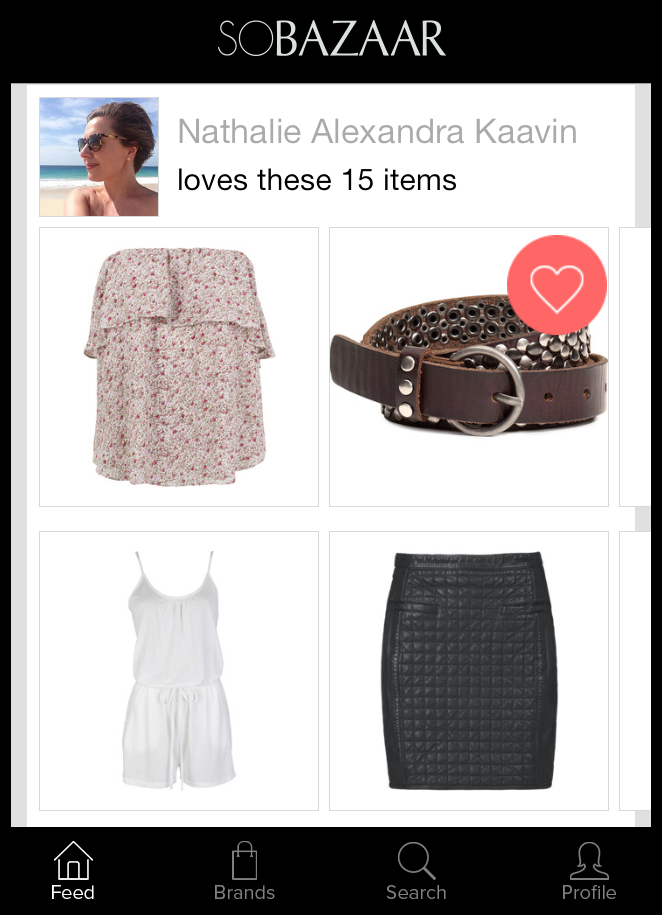
\includegraphics[height=1.5\linewidth]{image/SoBazaarfeed.png}
  \end{minipage}
  \hspace{.02\linewidth}
  \begin{minipage}{.3\linewidth}
        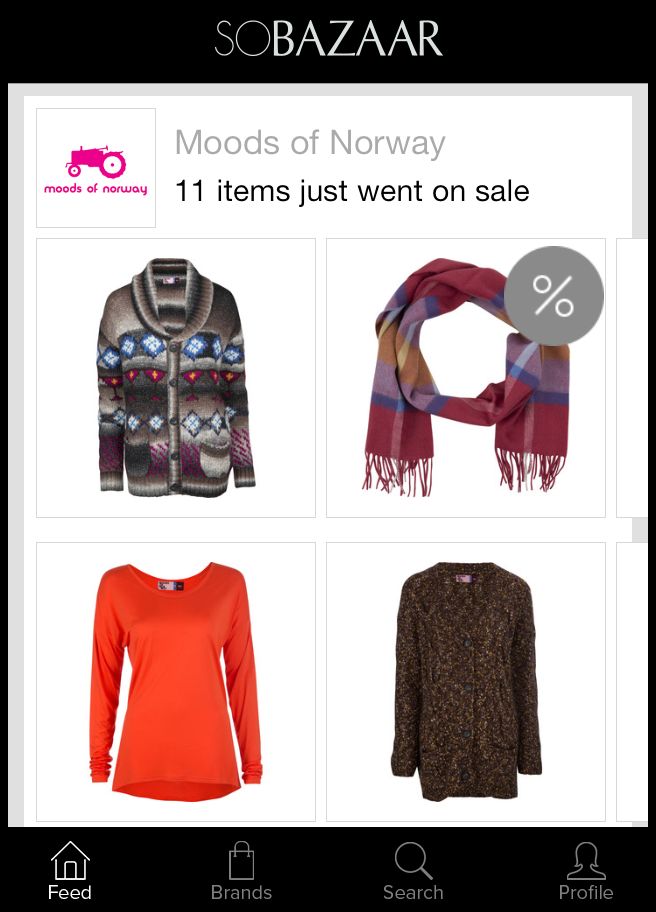
\includegraphics[height=1.5\linewidth]{image/SoBazaarsale.png}
  \end{minipage}
  \hspace{.02\linewidth}
  \begin{minipage}{.30\linewidth}
      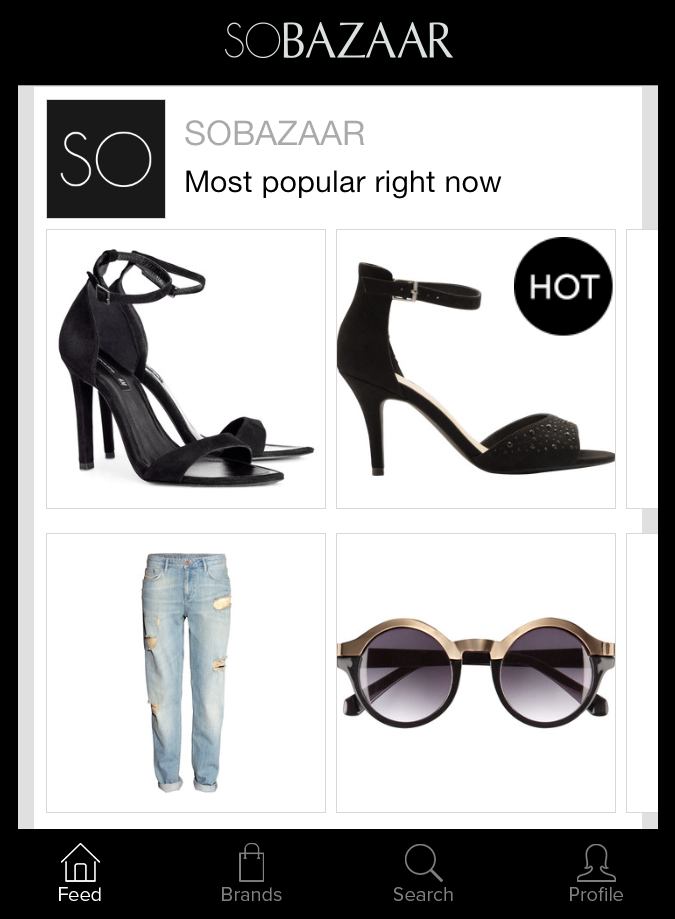
\includegraphics[height=1.5\linewidth]{image/SoBazaarmostpop.png}
  \end{minipage}
  \caption[SoBazaar newsfeed screenshots - version 0.5.1]{Screenshots from the
  SoBazaar newsfeed.}
  \label{figure:SoBazaarfeed}
\end{figure}

Users are also able to browse \textit{by brand} or storefront, as shown in the
leftmost screenshot below. A storefront is different from a brand-store by
combining products from a variety of brands into categorical sales or
\textit{packages} such as \textit{«summer sale»}. One of these storefronts are
coined \textit{Editor's picks}, which as we have mentioned, are curated by
professionals. If a brand or storefront is clicked one is taken to a custom
listing, presenting all products available together with their price and
optional status such as \textit{Hot} or \textit{New}.

\begin{figure}[H]
  \centering
  \begin{minipage}{.30\linewidth}
  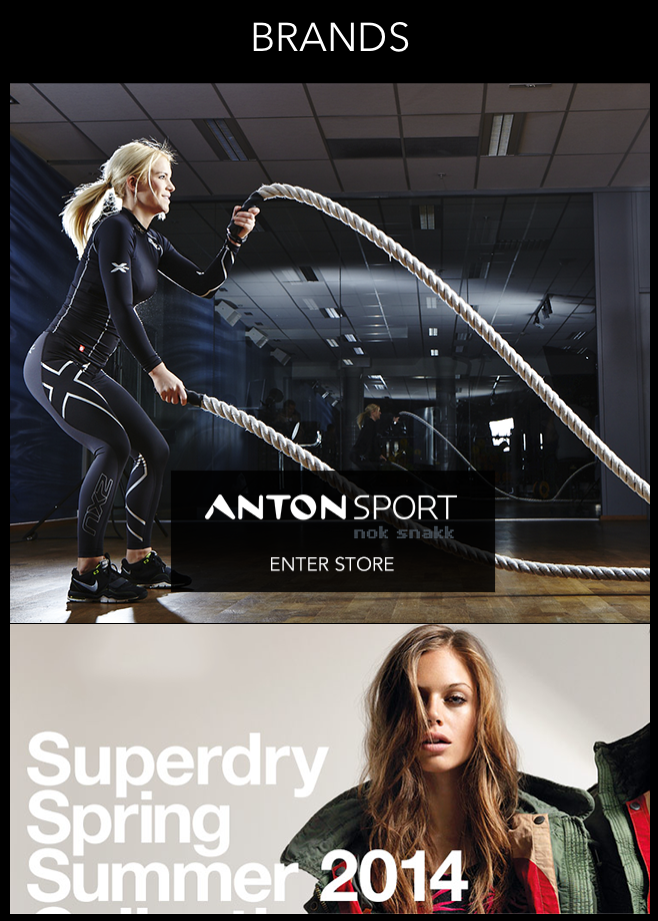
\includegraphics[height=1.5\linewidth]{image/SoBazaarbrands2.png}
  \end{minipage}
  \hspace{.02\linewidth}
  \begin{minipage}{.3\linewidth}
    
\includegraphics[height=1.5\linewidth]{image/SoBazaareditor.png}
  \end{minipage}
  \hspace{.02\linewidth}
  \begin{minipage}{.3\linewidth}
      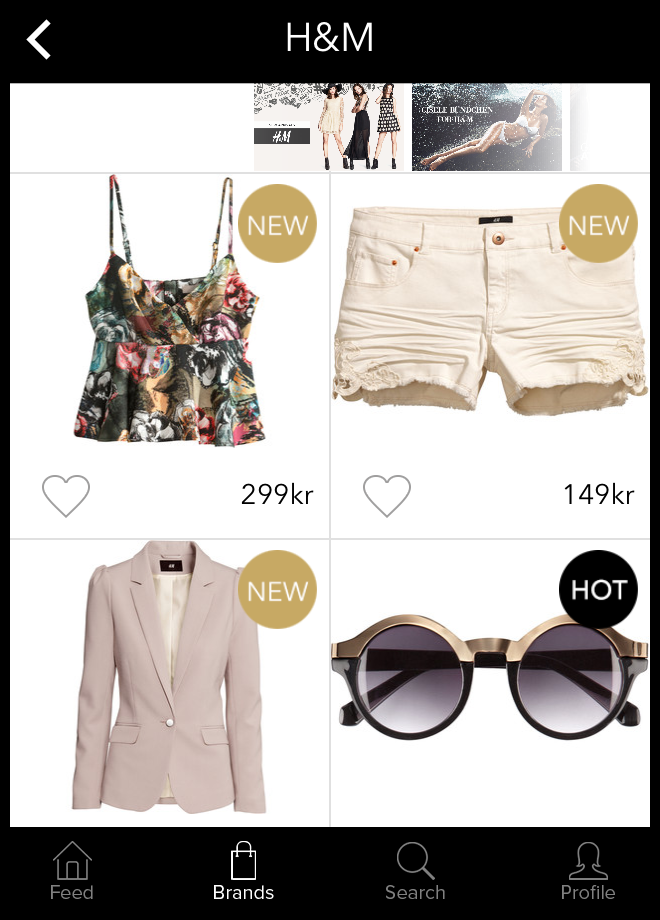
\includegraphics[height=1.5\linewidth]{image/SoBazaarStore.png}
  \end{minipage}
  \caption[SoBazaar storefront screenshots - version 0.5.1]{Screenshots from the SoBazaar Application. From the left to right: the brand browser, editors picks and the H\&M storefront}
  \label{figure:SoBazaarfeed2}
\end{figure}

From the product screen you can choose to buy the item, being redirected to an
external online shop for completing the purchase. The product screen currently
features a \emph{«People who like this also love»} section, in addition to show
other products from the same store. Clicking the map marker a map showing
nearby physical stores selling the item is expanded. Furthermore, the
info-button yields a more detailed description of the product and pressing the
rightmost arrow one has the possibility of sharing the item with friends via.
various social networks. The application also features a personal page for
earlier saved or \emph{wanted} items, named \textit{My love list}. Finally, the
application supports simple search queries on product descriptions, titles and
brand names. As can be seen from the rightmost image it is also possible to
filter the results by status, brand and category (type of attire).

\begin{figure}[H]
    \centering
    \begin{minipage}{.30\linewidth}
          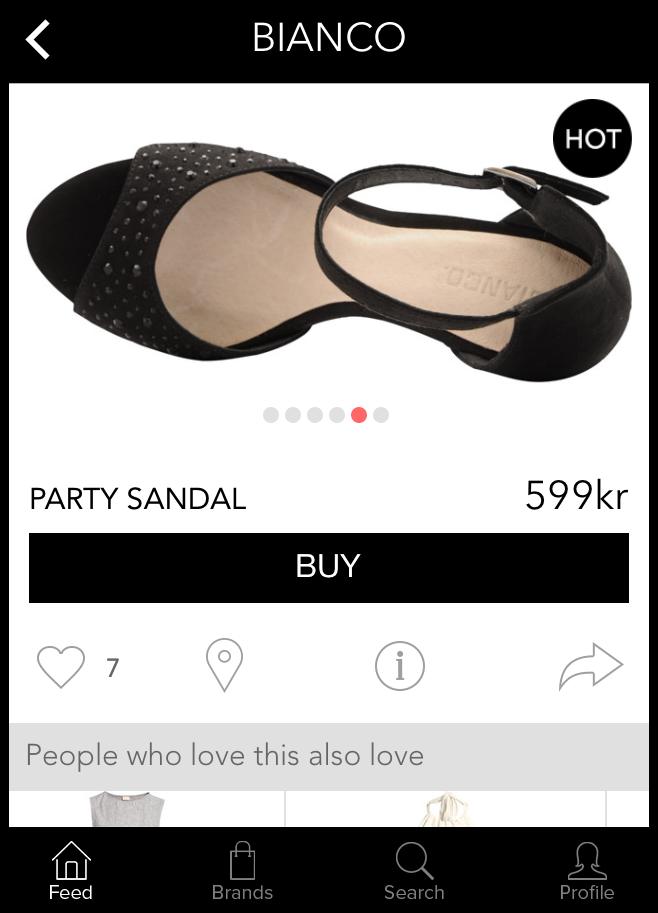
\includegraphics[height=1.5\linewidth]{image/SoBazaarproduct.png}
    \end{minipage}
    \hspace{.02\linewidth}
    \begin{minipage}{.3\linewidth}
      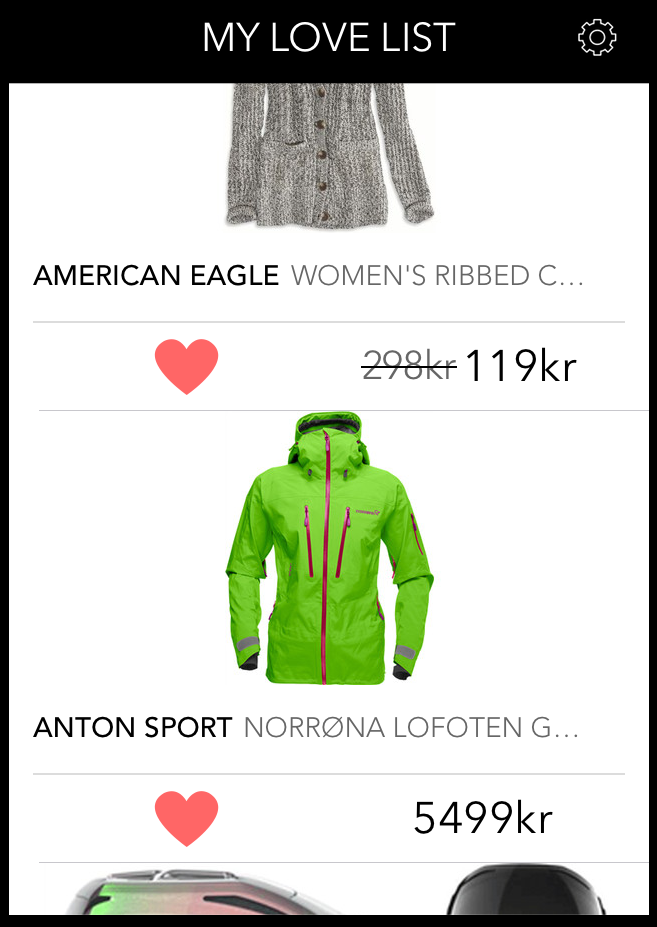
\includegraphics[height=1.5\linewidth]{image/SoBazaarlovelist.png}
    \end{minipage}
    \hspace{.02\linewidth}
    \begin{minipage}{.3\linewidth}
        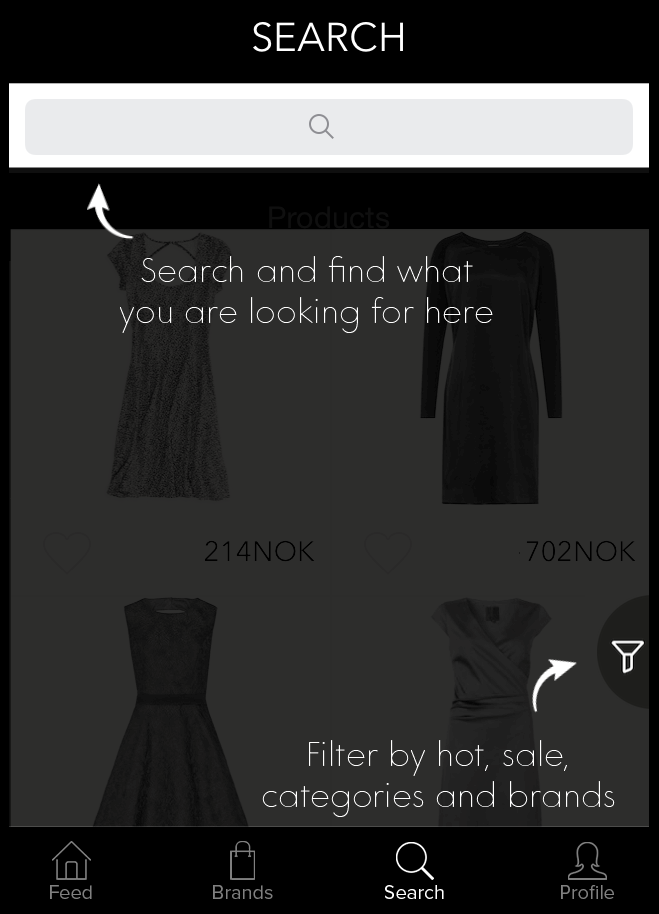
\includegraphics[height=1.5\linewidth]{image/SoBazaarsearch.png}
    \end{minipage}
    \caption{Screenshots showing product details, love list and search functionality}
    \label{figure:SoBazaarfeed3}
\end{figure}

The application is currently in a beta phase and is planned for a final release after the summer.

\section{Preprocessing}
\label{sec:preprocessing}

In data mining, preprocessing is an important procedure which lays the
foundation for further data analyzation. The saying \emph{garbage in, garbage
out}~\cite{GIGO} especially applies here, as the quality of input data can make or
break the final results. This is due to a variety of reasons, ranging from
non-complete raw-values, events outside target groups or outliers having
user-beahviours which makes learning stereotypical patterns impossible.

The following pre-processing steps were performed before continuing to analyze
the dataset:

\begin{itemize}
  \item Anonymization of all personal information, including positional data.
  \item Removal of all events made in test or staging environments.
  \item Removal of suspicious users having activity levels multiples above
  normal. The majority of these events were made in the early phase of the
  application.
\end{itemize}

As part of the preprocessing, a unique \textit{session identfier} field was
added to the data, indicating which events were done in the same timespan
without closing the application. This, as we will see in later sections helps
us understand multiple usage patterns.

\section{Dataset Overview}

The data from SoBazaar is based on all actions, also called events, made by the
users. They can range from accessing a storefront, scrolling the page or
purchasing a product. Combined, they form the basis of which we develop all
techniques in this thesis. When an event is triggered a set of information is
stored regarding the event, describing the \textit{context} of which the event
was fired, where the most relevant event-metadata, in terms of recommender
systems, are presented in the table below.

\begin{table}[H]
    \centering
    \begin{tabular}{l p{11cm}}
        \toprule
        Variable     & Explanation   \\
        \midrule
        \emph{product\_id}        & Unique id of the item on which the event
                                    was triggered \\
        \emph{user\_id}           & Unique id of the user who triggered the event \\
        \emph{event\_id}          & What kind of event was
                                  triggered~\tablefootnote{Complete list of the
                                  different types of events can be found in
                                  table~\ref{table:completeEventData}} \\
        \emph{price}              & The price (in NOK) of the item \\
        \emph{retailer\_brand}    & Unique id of the item retailer. A retailer
                                    is a distributer of products, such as H\&M,
                                    Cubus or Moods Of Norway \\
        \emph{storefront\_id}     & The storefront id of the storefront entered.
                                    A \textit{retailer\_brand}s can have multiple
                                    \emph{store\_fronts}. \\
        \emph{event\_location}    & The location of the user when the event was triggered \\
        \emph{ts}                 & Unix timestamp in milliseconds of when the event was triggered \\
        \emph{session}            & Which session number the event belongs
                                  to~\tablefootnote{This is the value added in the preprocessing
                                  phase~\ref{sec:preprocessing}. For two events to end up in the same
                                  session, the event has to be triggered within a certain period of time,
                                  and both be after the same application started-flag} \\
      \bottomrule
    \end{tabular}
    \caption[Event Metadata]{Metadata collected from an event. The complete list can be found in table~\ref{table:completeEventData}}
    \label{table:eventData}
\end{table}

These events are used to derive information regarding both users and products
-- and combined and structured they form what we call \textit{implicit
feedback}. After preprocessing the data we look at some key figures, in order
to better understand its properties.

    \begin{table}[H]
        \centering
        \begin{tabular}{l l}
            \toprule
            Attribute       & Count   \\
            \midrule
            Total number of product events  &    35324 \\
            Unique users ids    &    1532 \\
            Unique item ids     &    5688 \\
            Unique storefronts  &    144~\tablefootnote{A storefront is a access point, with different clusterings of items. Stores can have multiple storefronts} \\
            Unique retailer brands  &    22 \\
            \hline
            Item clicks     &    21400 \\
            Item wants  &    12436 \\
            Item purchases  &    1488 \\
            \hline
            First event & Mon, 07 Oct 2013 10:59:57 GMT \\
            Last event & Mon, 19 May 2014 22:51:19 GMT \\
            Lifetime of data & 224 days \\
            \hline
            Average item click count per user   &    13.9686 \\
            Average item want count per user    &    8.1174 \\
            Average item purchase count per user    &    0.9712 \\
            \hline
            Average user interaction count per item     &    6.2102 \\
            Average item interaction count per user     &    23.0574 \\
            Median item interaction count per user  &    7.0 \\
            \bottomrule
        \caption[Dataset summary]{Overview of the key figures in the SoBazaar dataset}
        \label{table:datasetSummary}
        \end{tabular}
    \end{table}

As seen from table~\ref{table:datasetSummary} the average amount of
\emph{purchases} per user are below one. Using purchase information alone to
make recommendations will therefore in most cases render the recommendations
incomplete. If one or more users have more than one purchases, then some users
will of course have none purchases. Making personalized recommendations for
these users will then be unattainable.

\emph{Clicks} and \emph{wants} on the other hand have a much higher occurrence.
These two events together with \emph{purchases} tops a count of 20 on average
per user, and opens for the possibility of more dense personalized
recommendations, but the data is still rather sparse.

\section{Visualizations and analysis}
    % New graphs when/if:
    % Price range of items in stores
    % unique Stores count for users
    %     price span for user
    %         Timespann of sessions for users (avg, max, min)
    %         Events per session (avg, max, min)
    %         Item viewtime for user in session
    %         Stores visited per session
    %         revisit time of items for user
    %         relationship with view, want and purchase
    %         time of session over lifetime of app
    %         user preferred price in session
    %         price vs view, want and purchase
    %         avg viewtime for an item (i know)
    %         Similarity of user favorite store, items viewed and items wanted?
    %         time of session over lifetime of app for all users (slope-style)
    % check for price distribution based on location.
    % make price user graph
    % price for store dist

In this section, in accordance to research \textbf{goal G1} a thorough analysis
of the SoBazaar data will be carried out. By carefully crafted visualizations,
patterns emerge and we gain valuable knowledge of which we share the
consequences, both in terms of recommender systems and limitations of this
thesis. In order, we inspect: user, product and time related properties found in
the data -- keeping in mind the table presented in the previous section
(Table~\ref{table:datasetSummary}).

\subsection{User properties}

We start our analysis by trying to understand \textit{how} the users interact
with the application and to which degree we can use user-based features in
order ot make predictions. We do this by primarily looking at their
distributions with regards to events, purchases, sessions and their lifespan in
the application -- that is how well customers are retained.

\begin{figure}[H]
  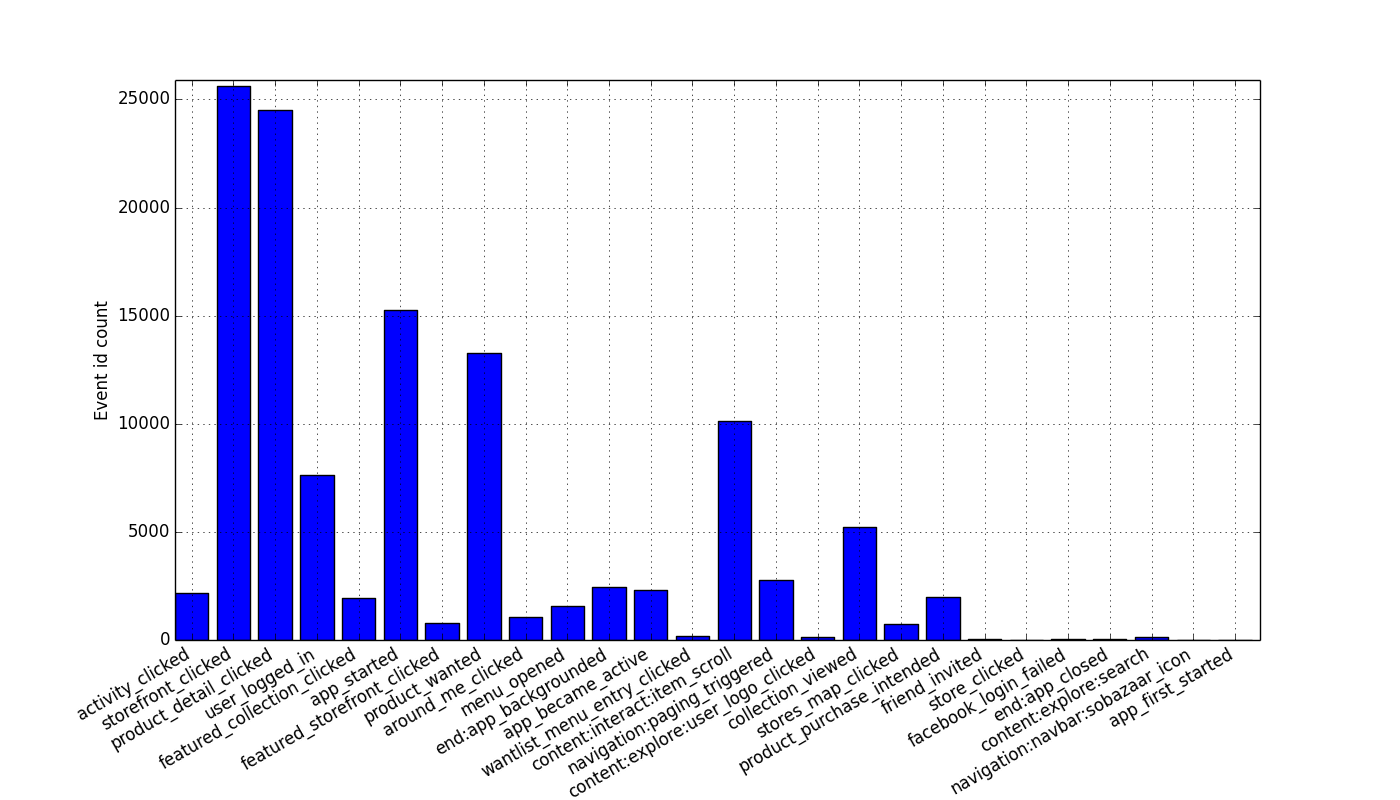
\includegraphics[width=5in]{image/event_iddistribution.png}
  \centering
  \caption{Event distribution}
\label{figure:eventIDDistribution}
\end{figure}

Here we see the count for each of the different events which can be triggered
in the SoBazaar application\footnote{With the exception of the event types with
a trigger count lower than 200, which are merged into on bar and labeled
\emph{other}}. As can be seen, the two events \emph{product\_detail\_clicked}
and \emph{storefront\_clicked}, are the two most common in the dataset. As
mentioned earlier in Section~\ref{sec:sobazaar-appication}, the
\emph{storefront} is the main access point to a set of products, and the high
values for this \emph{event\_id} is expected. The fact that accessing the
\emph{storefront} is the most occurring event, over clicking an item, indicates
that many users use the application primarily to browse through items, looking
at thumbnails, rather than accessing the actual item. This underlines the
importance of having good and presentable images, provide useful information
about the product in the overview (See Figure~\ref{figure:SoBazaarfeed}) where
price and status (\textit{New}, \textit{Hot} or \textit{On sale}) should be
easily accessible.

As we can see from Figure~\ref{figure:SoBazaarfeed3} it is possible to indicate
that you want an item (\textit{product\_wanted}) by clicking the heart-icon,
and without accessing the acutal item -- that is sending a
\textit{product\_detail\_clicked}. Hence, although the number of wants are half
the number of clicks, it does not imply that half of the users clicking an item
wants it. This does not hold true for purchases, where one has to click the
item before sending the \textit{product\_purchase\_indtended} event -- thus we
can conclude that 6.9\% of all clicks progress into an \textit{intended}
purchase.

Some of the events shown above are newly added to the application, and the data
for these (e.g. \textit{content:interact:item\_scroll} needs to mature more in
order to draw certain conclusions.

In the title of this thesis we proclaim that the dataset is \textit{extremely
sparse} and this can be confirmed by looking at the distribution of events per
users, below.

\begin{figure}[H]
    \centering
    \begin{subfigure}{.5\textwidth}
        \centering
        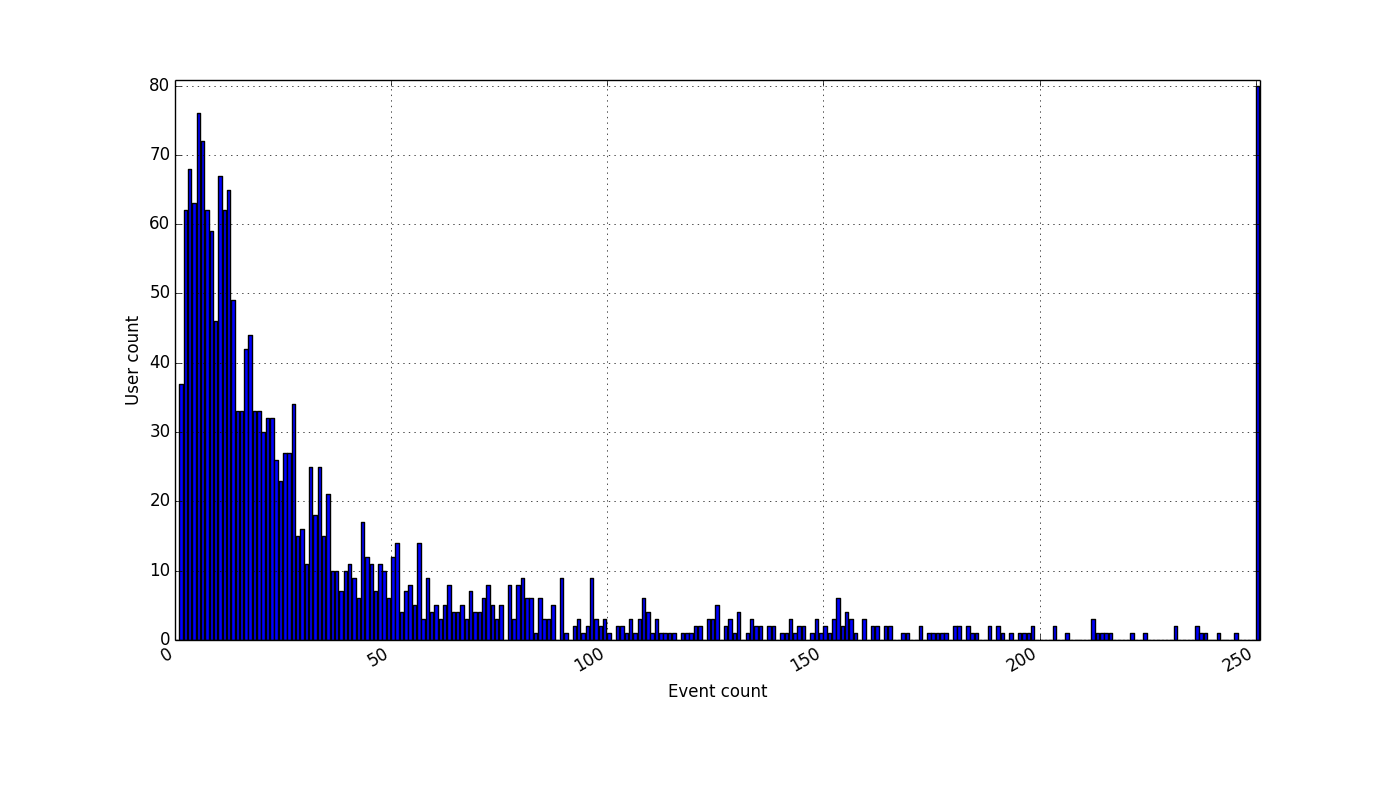
\includegraphics[width=\dualGraphWidth]{image/user_iddistribution.png}
        \caption{Distribution of events on users}
        \label{fig:userEventDist}
    \end{subfigure}%
    \begin{subfigure}{.5\textwidth}
        \centering
        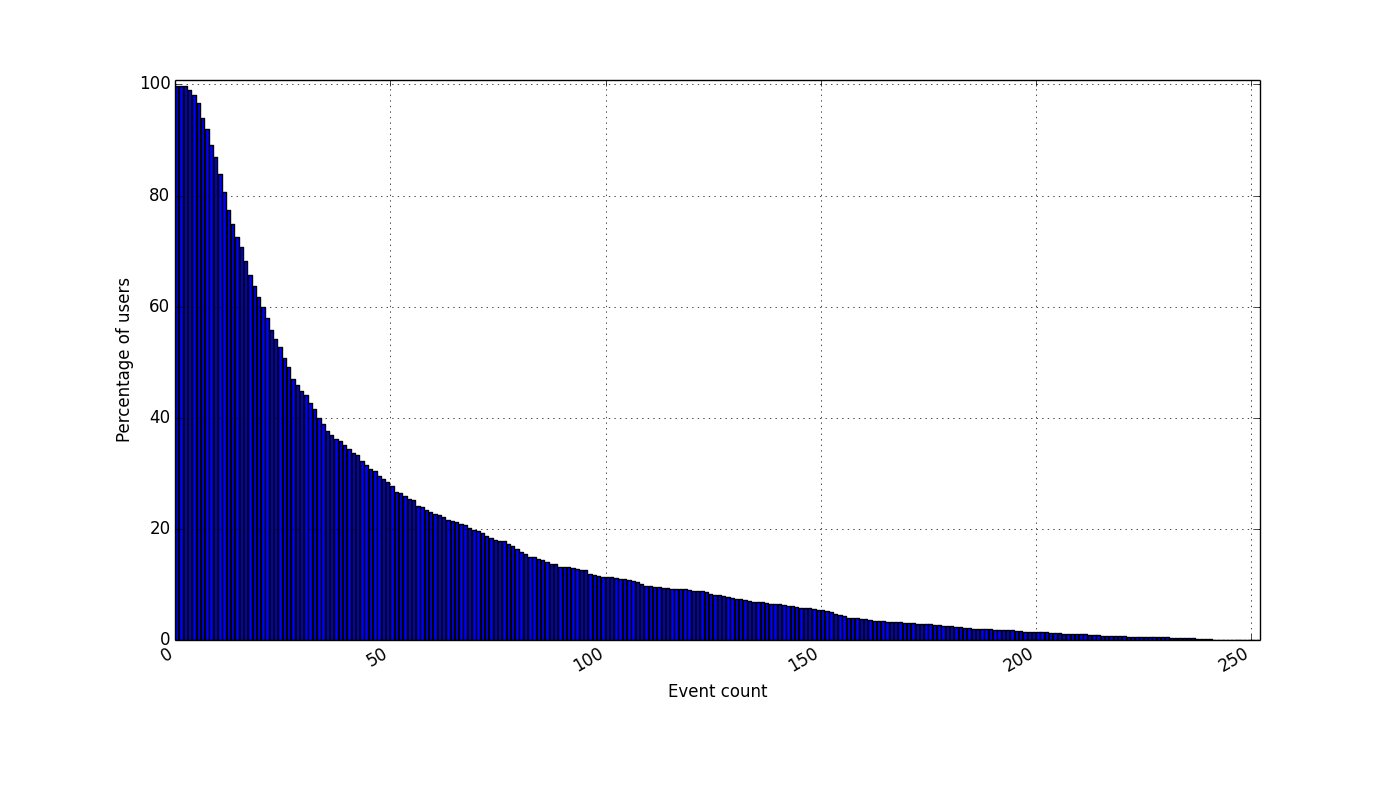
\includegraphics[width=\dualGraphWidth]{image/user_idcumdistribution.png}
        \caption{Cumulative distribution of events on users}
        \label{fig:userEventCumDist}
    \end{subfigure}
    \caption{Distribution of events per user}
\end{figure}

We can see that this figure confirms our title. In
Figure~\ref{fig:userEventDist} the majority of users have been observed
doing less than 10 events, and Figure~\ref{fig:userEventCumDist} confirms this
by presenting the cumalative graph where, 78\% of the users have 50 events or
less, with an average of 5 events per user. Note that we here look at
\textit{all event types}, not only those where the user interact with items. As
we, in our proposed system, do not use non-item events for neither recommending
nor generating implicit ratings, we now look at the event distribution when
only the three item events \textit{product\_detail\_clicked},
\textit{product\_wanted} and \textit{product\_purchase\_intended} are issued.
We do include the distribution above however, to show how sparse the data is --
both in terms of product interaction, but also application interaction.

\begin{figure}[H]
    \centering
    \begin{subfigure}{.5\textwidth}
        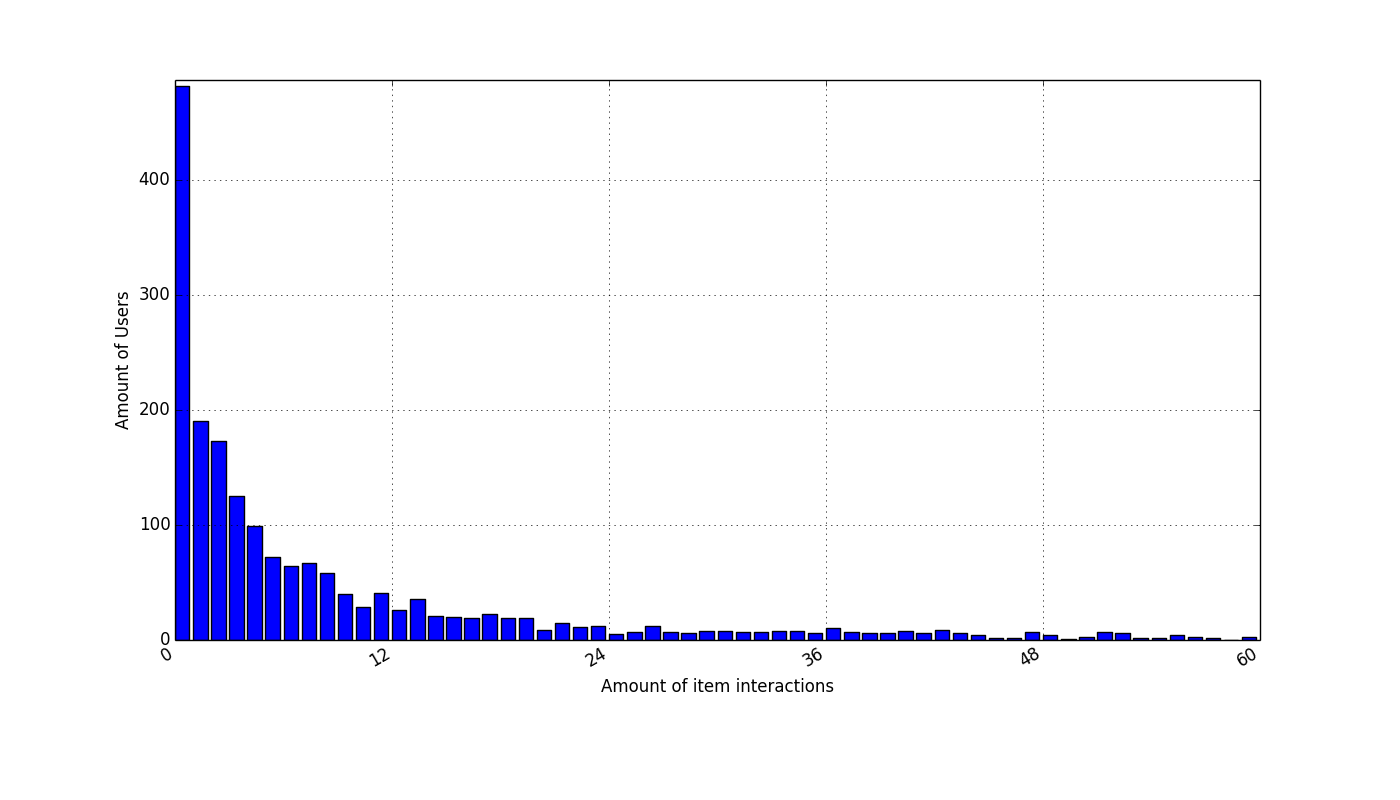
\includegraphics[width=\dualGraphWidth]{image/ratingsPerUserdistribution.png}
        \centering
        \caption{Count of item interactions for users}
        \label{fig:ratingsPerUser}
    \end{subfigure}%
    \begin{subfigure}{.5\textwidth}
        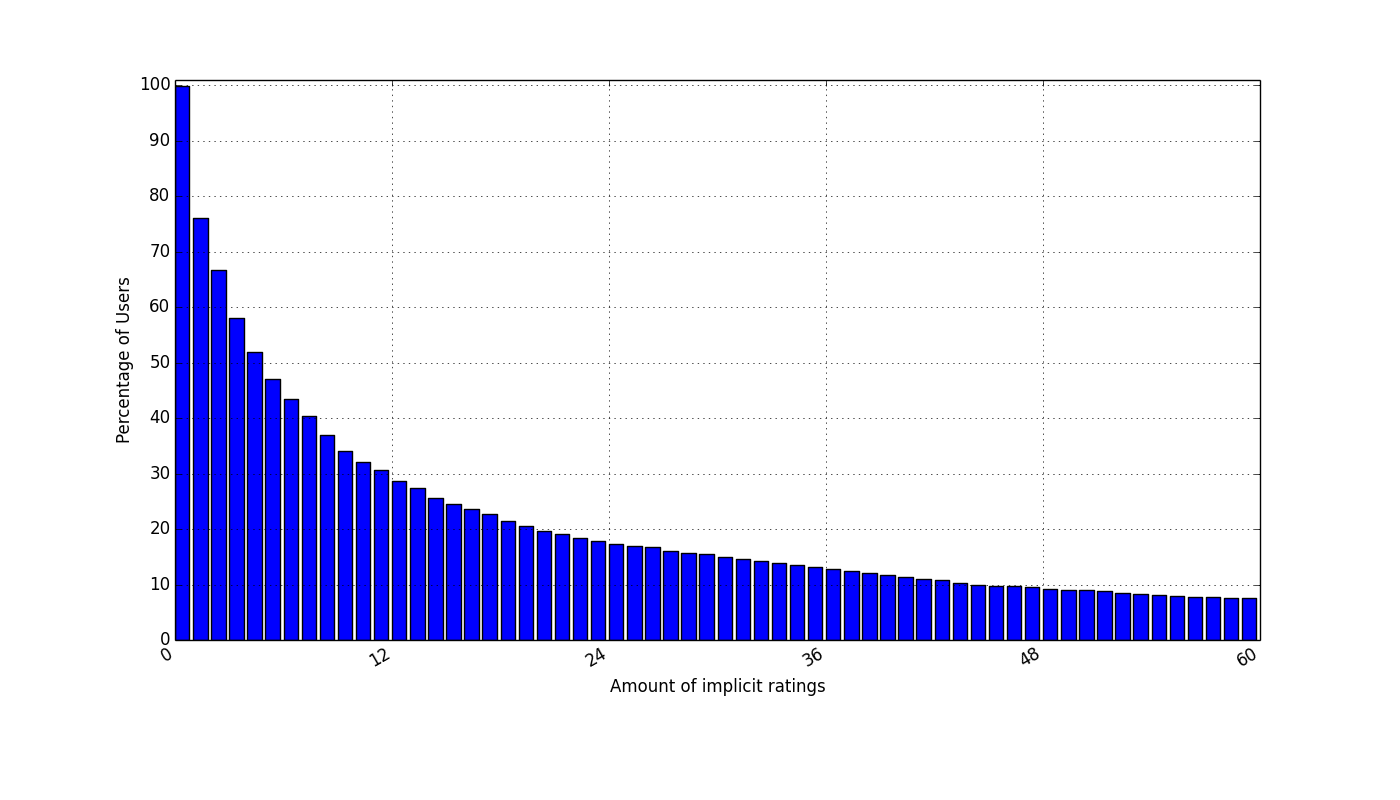
\includegraphics[width=\dualGraphWidth]{image/ratingsPerUsercumdistribution.png}
        \centering
        \caption{Cumulative count of item interactions for users}
        \label{fig:ratingsPerUserCum}
    \end{subfigure}
    \caption{Number of product interactions per user}
\end{figure}

In the figures above we see the number of product interactions per user, where
the following key charecterstics are apparent:

\begin{itemize}
  \item Over 20\% of all users have never interacted with an item (leftmost bar
  in Figure~\ref{fig:ratingsPerUserCum})
  \item 90\% of all users has 60 or fewer item interactions, this is set as
  cut-off point in both figures.
  \item 70\% percent of the users has 12 or fewer item interactions.
  \item The average number of item-interactions per user is, per
  Table~\ref{table:datasetSummary},
  $23.05$, however as a few users skew this number a more accurate measure is
  the median which yields $7.0$ interactions per user.
\end{itemize}

Consequently, although the data extremely sparse the fact that the majority of
the users have in \textit{some way} interacted with at least one item, opens
for the possibility of connecting users based on their item interactions and
making rudimentary recommendations.

Up until now, we have seen how the users have interacted with both the
application and products, however we gain a better understanding of the domain
by also studying user patterns such as how often the application is used and
the lifespan of user-accounts.

\begin{figure}[H]
  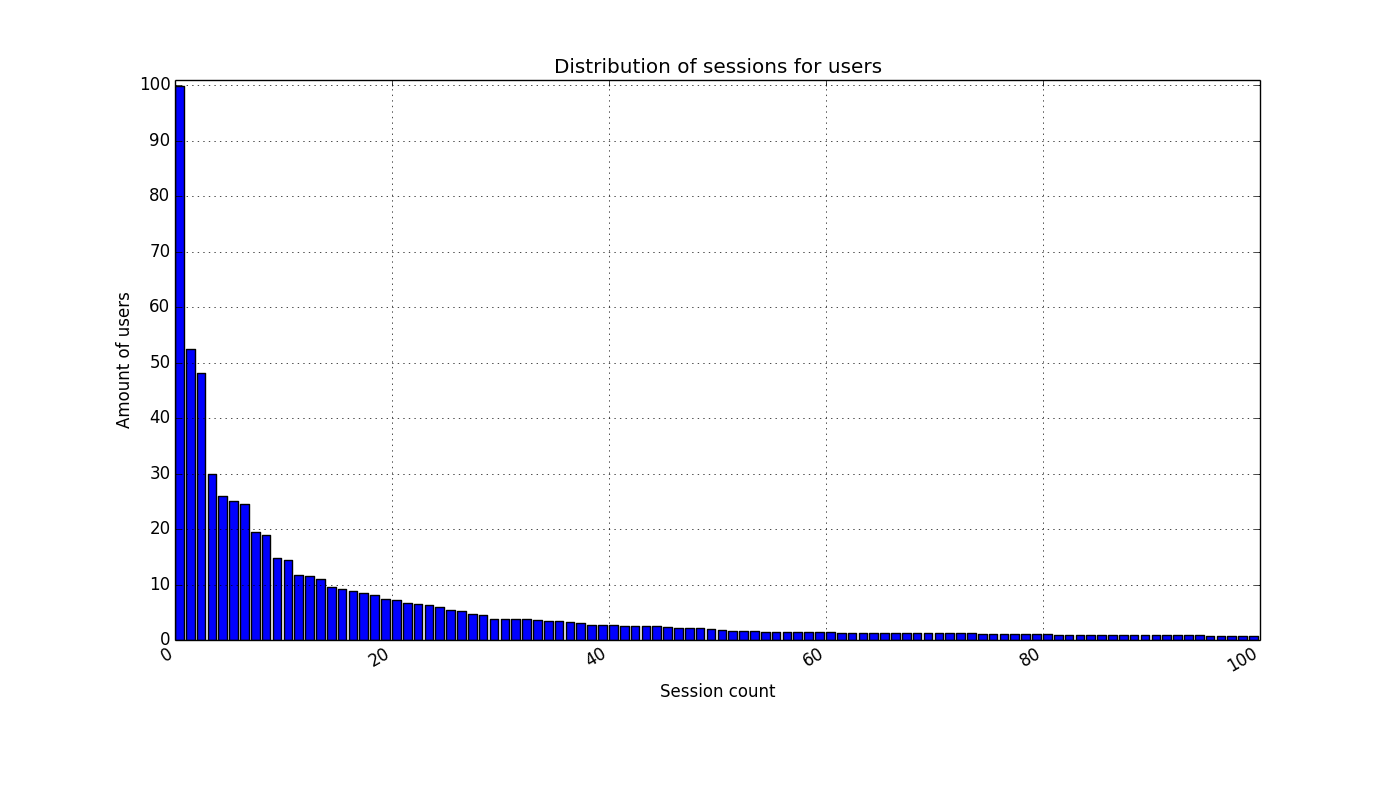
\includegraphics[width=5in]{image/sessiondistribution.png}
  \centering
  \caption{Distribution of sessions for users}
  \label{fig:sessCountDist}
\end{figure}

As seen from the above figure, more than 90\% of the users have a session count
of 20 or less, in addition almost 25\% of all users has only registered
\textit{one} interaction in the lifetime of their account. Taking this
calculation further, approximatly 50\% of the users has 6 interactions or fewer, all
evidence to strengthen the sparsity claim made in the title of this thesis.

The low number of sessions leads us to look at account lifetime, where we
define the lifetime of a user as the length between the first and last
registered event recorded.

\begin{figure}[H]
  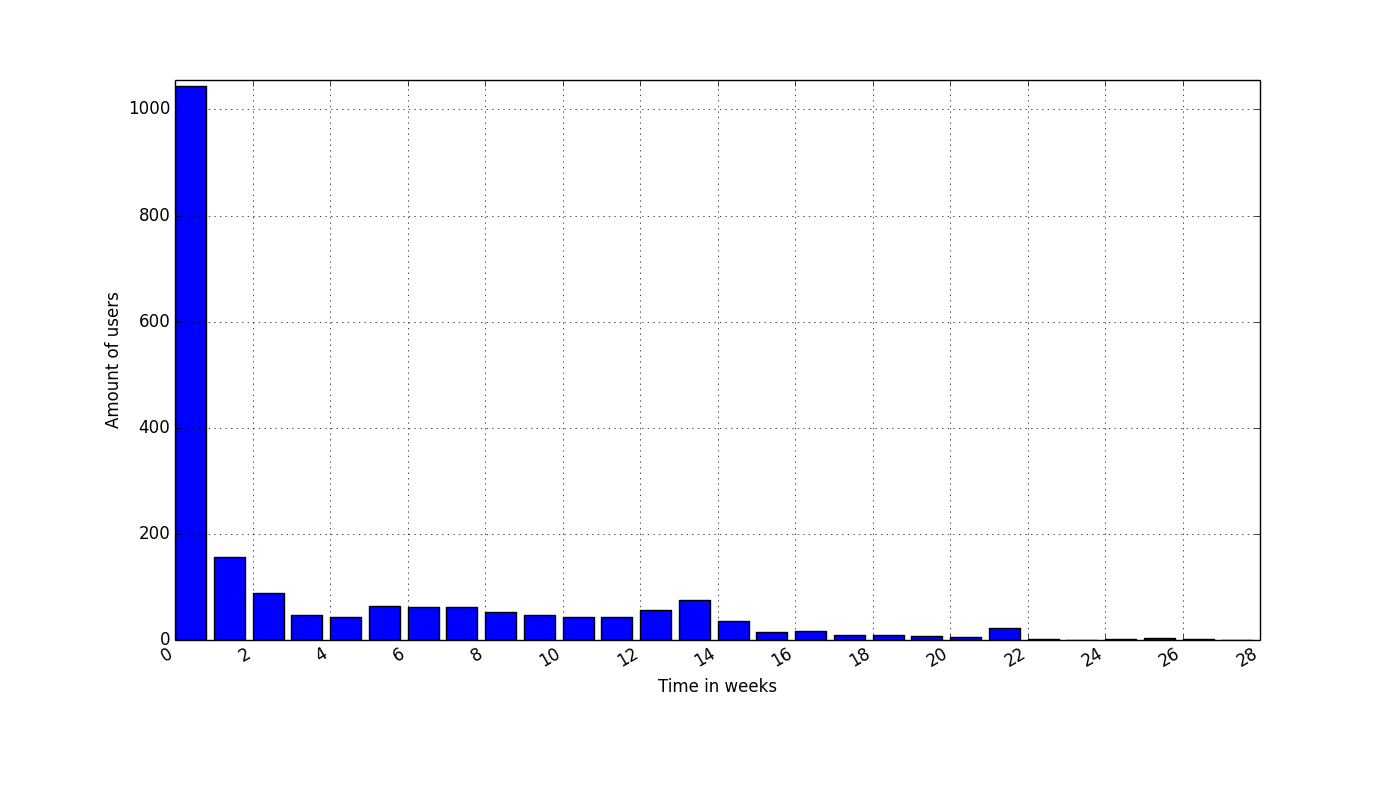
\includegraphics[width=5in]{image/userTimespansdistribution.png}
  \centering
  \caption{Distribution of user account lifetime}
  \label{figure:userTimespandist}
\end{figure}

From this figure we conclude that over half of the users have a lifespan of
less than a week, in many ways confirming the user effects seen in
Figure~\ref{fig:sessCountDist}, as many users use the application a few times
and never open it again. Using this knowledge we observe how important it is to
based on demographics and \textit{cold-start methods} recommend relevant items
from day one.

One might however argue that a short lifespan does not necessarily yield low
activity, and in order to disprove this claim we map the average lifespan at
the Y-axis and combine it with the event count of users on the X-axis.

\begin{figure}[H]
  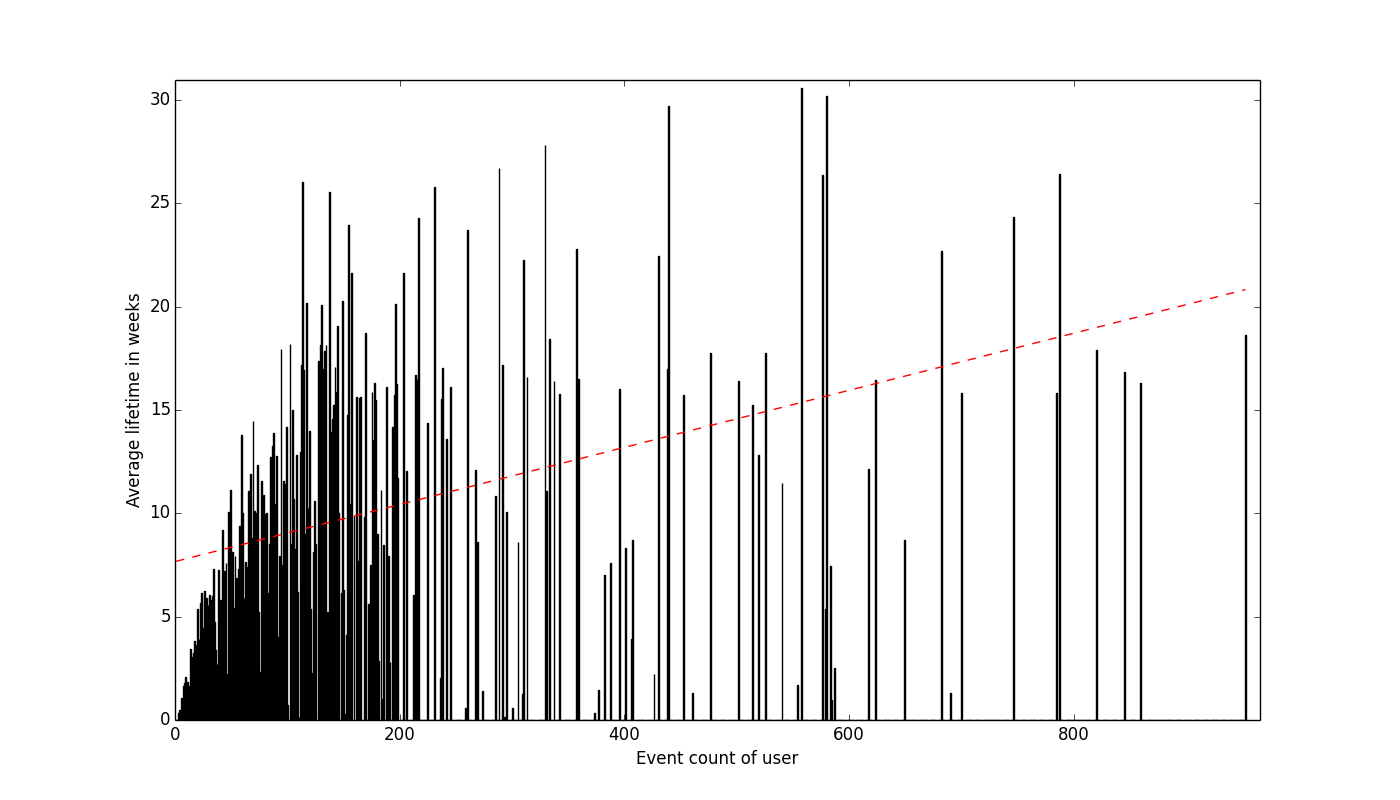
\includegraphics[width=5in]{image/avglifetimeoncountuser.png}
  \centering
  \caption{Average lifetime of user accounts sorted on event count}
  \label{figure:avglifetimeoncountuser}
\end{figure}

As seen from the tendency line, a longer lifespan of a user yields a larger
probability of a higher event count. Based on our findings at this point we can
thus conclude that the data is sparse and many users have only used the
application a few times, without coming back.

Continuing, we want to learn more about the user demographics and therefore use
the location provided with each event to map the locations of all users in
Norway, as shown below.


\begin{figure}[H]
  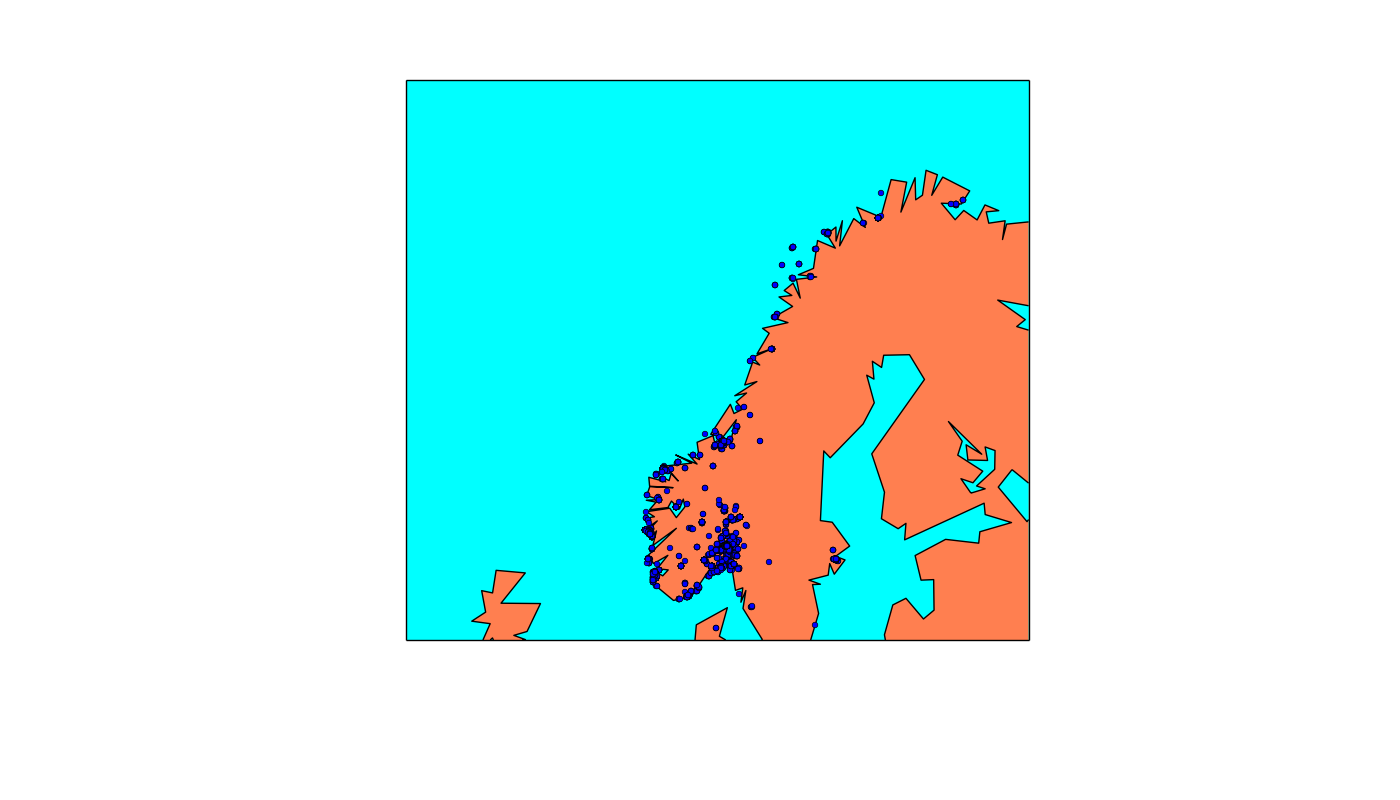
\includegraphics[width=5in]{image/simpleGeoPlotNorway.png}
  \centering
  \caption{Primary event locations in Norway}
  \label{figure:croppedGeoplot}
\end{figure}

The locations of all users in Norway, shows that users from the whole country
are using the application and they correspond roughly to the population
distribution as well -- this has the pleasant side-effect that making
predictions based on demographics, may prove successful. However, experiments
must the done in order to see to which degree one can make generalizations in
city-centers, where most of the acitivity are coming from.

\subsection{Product properties}

Having covered many of the properties found in the users of SoBazaar, we move
our attention to the products to see how they are interacted with and if we
gain any valuable knowledge which might lead us to better undertstand the
domain. First we will look at the price distribution, before moving on to see
how evenly distributed the product events are, and finally we delve more into
detail on \textit{storefronts} and their effect on the dataset.

\begin{figure}[H]
  \centering
  \begin{subfigure}{.5\textwidth}
      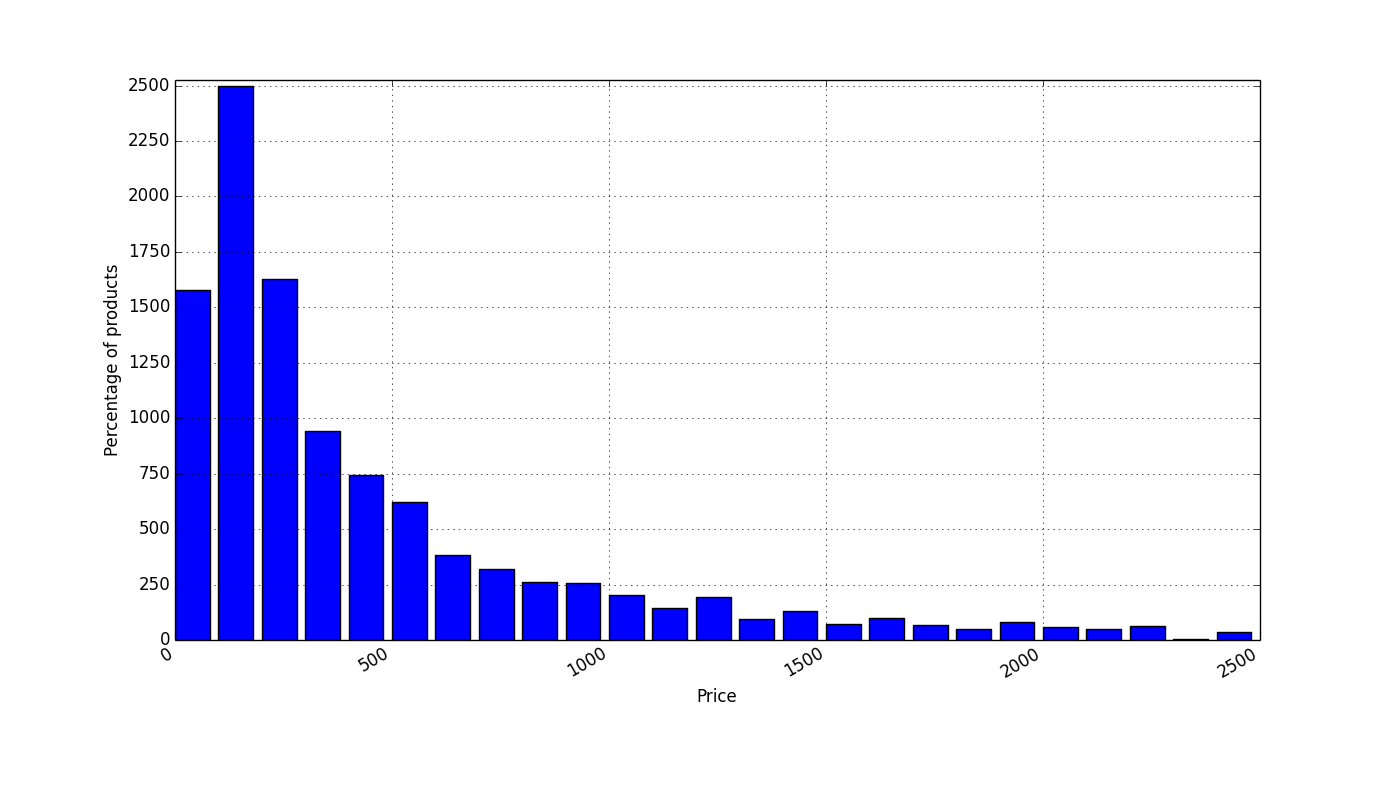
\includegraphics[width=\dualGraphWidth]{image/priceDistributiondistribution.png}
      \centering
      \caption{Price distribution of products}
      \label{figure:pricePerProduct}
  \end{subfigure}%
  \begin{subfigure}{.5\textwidth}
      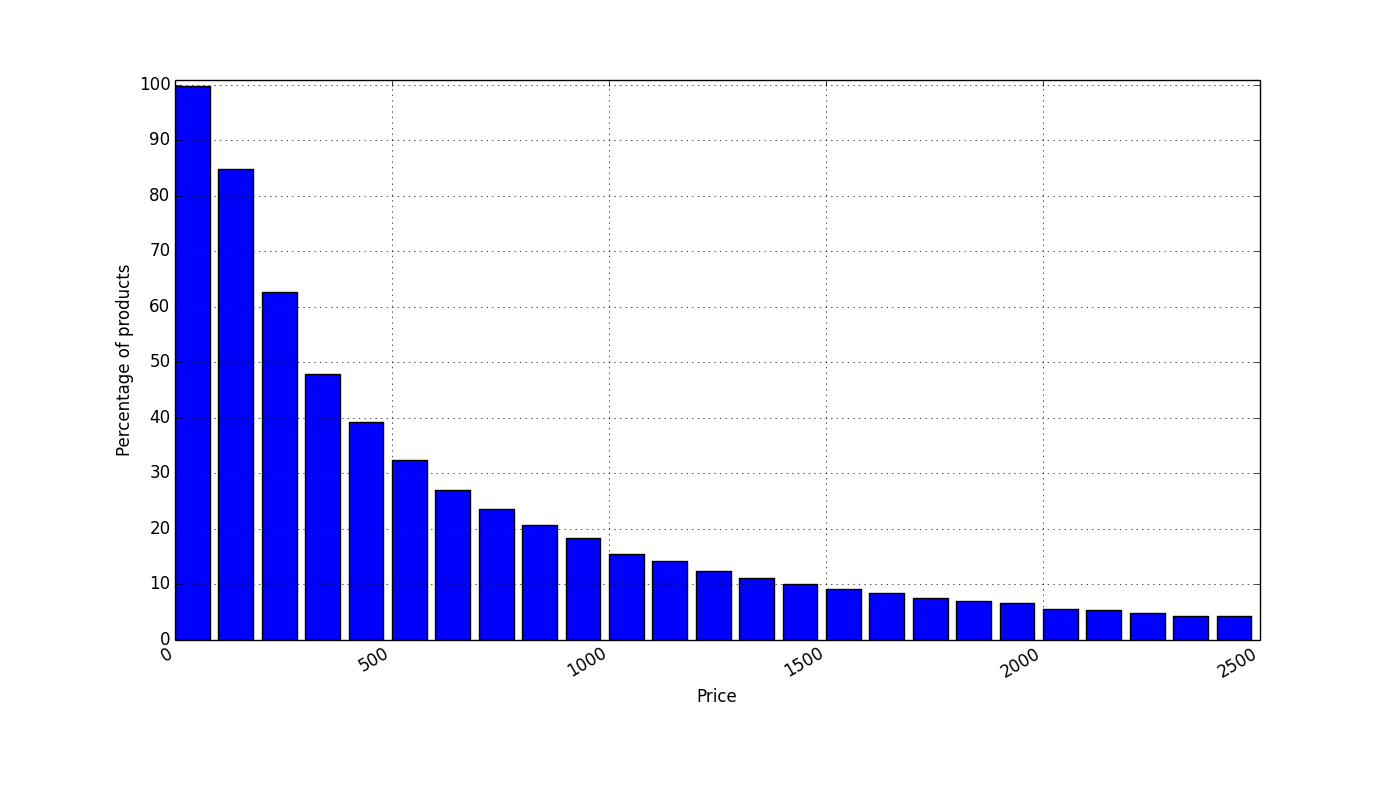
\includegraphics[width=\dualGraphWidth]{image/cumpriceDistributiondistribution.png}
      \centering
      \caption{Cumulative price distribution of products}
      \label{figure:pricePerProductCum}
  \end{subfigure}
  \caption{Figures presenting the distribution of price for the items i SoBazaar}
\end{figure}

From the above figures we note that the majority of items (82\%) have a price
lower than 1 000 NOK. There is a definite peak around 200-300 NOK, which
correlates with the median price for items being 299 NOK.  Still, the
variations seen in Figure~\ref{figure:pricePerProduct} are big and this is a
good thing as it can help us differentiate on users based on their price
preferences.

Can we, however, make the same differantiation based on popularity? We have
seen that each item in average has $6.21$ interactions
(Table~\ref{table:datasetSummary}, but as seen below these are not evenly
distributed among the products.

\begin{figure}[H]
  \centering
  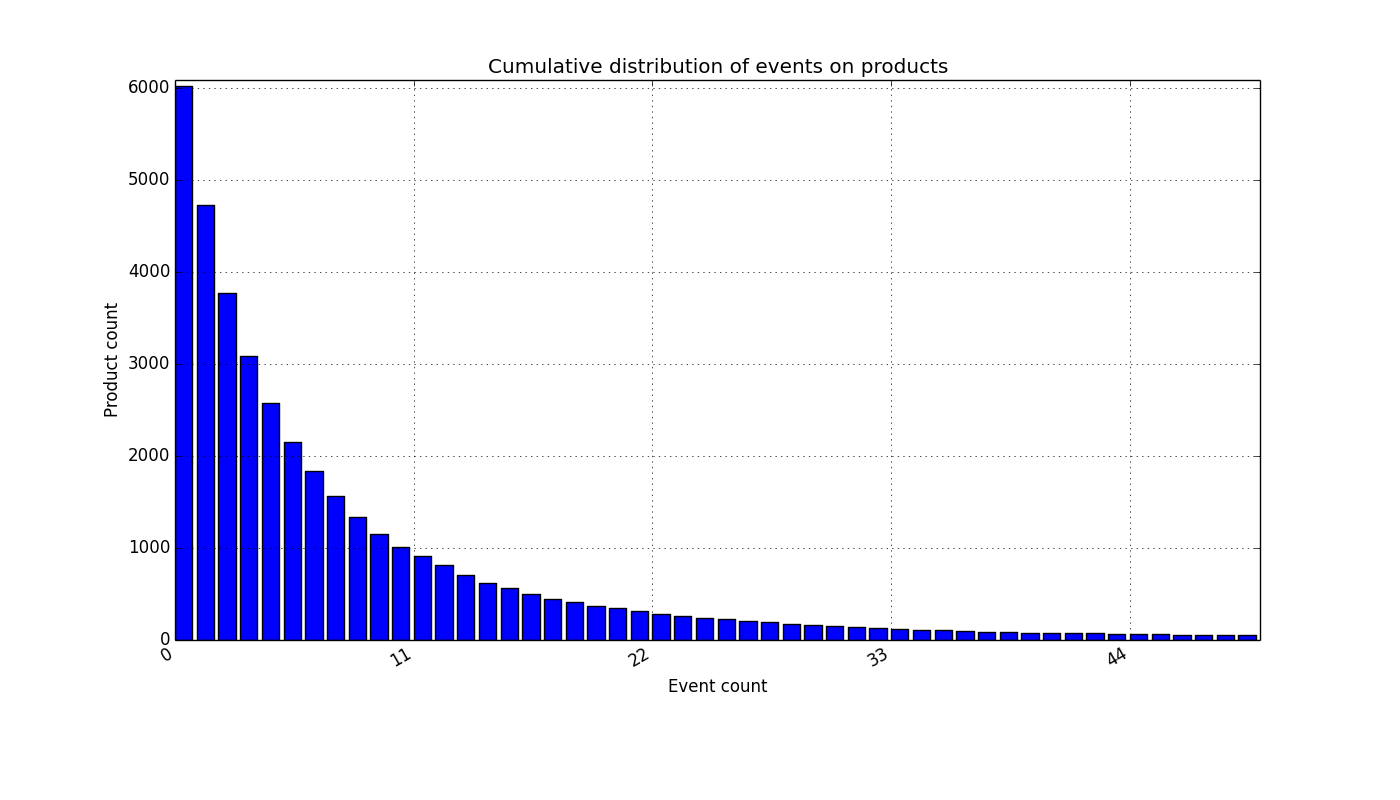
\includegraphics[width=\dualGraphWidth]{image/product_idcumdistribution.png}
  \label{figure:eventsPerproductCum}
  \caption{Cumulative count of events on products}
\end{figure}

80\% of the products only have an interaction count of 10 or less, where
interaction count is \emph{product\_detail\_clicked}, \emph{product\_wanted}
and \emph{product\_purchase\_intended}.  This means that there will not be more
than 10 events for the majority of the items, with no more than 10 datapoints
to connect with other items for the majority of the items, recommendations done
through connecting items to other items through item interaction, might prove
problematic.

When the majority of the events only has 10 events and there are over 6 000
items and 2 000 users, the probability that multiple users have interacted with
similar items will be marginal, but promotes the importance of utilizing all
the feedback to bolster the recommender.

\subsubsection{The Pareto principle and Long tail on interactions}

In e-commerce the distribution of sales or product interactions can often be
described by the Pareto principle and the phenomenon of \textit{long tail}
which states that roughly 80\% of the effects come from 20\% of the causes.
Often the principle goes by the name of \textit{factor sparsity}, which
indicates that given a Pareto distribution one \textit{may} observe sparsity
issues. Whilst measuring the Pareto principle focuses on the \textit{head} of
the distribution (that is, where it is steepest), the \textit{long tail}
phenomenon targets the \textit{tail}. It states that the most frequently
occurring items represent less than 50\% of seen
occurrences~\cite{DBLP:journals/corr/abs-1203-4487}, thus by having a Long-tail
distribution, events are more evenly distributed compared to when Pareto yields
true.

In order to analyze these distributions we map our product interactions on the
Y-axis and sort our products by popularity on the X-axis -- grouped by the
popularity percentage, that is the 1\% most popular items equals 1\% of 5688,
in other words the 57 items.

\begin{figure}[H]
  \centering
  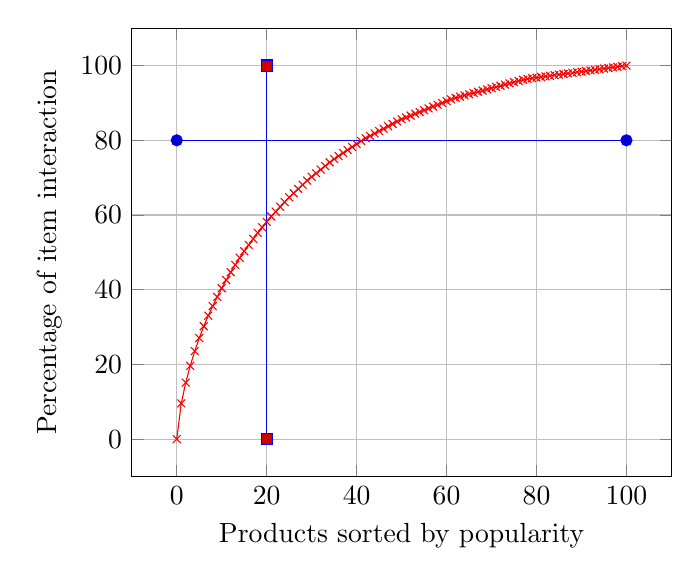
\begin{tikzpicture}
    \begin{axis}[
      xlabel=Products sorted by popularity,
      ylabel=Percentage of item interaction,
      grid=major,
    ]
    \addplot+[color=blue,sharp plot] coordinates
      {(0,80) (100,80)};
    \addplot+[color=blue,sharp plot] coordinates
      {(20,0) (20,100)};
    \addplot[color=red,mark=x] coordinates {
        (0.0, 0.0)
        (1.0, 9.576667138609656)
        (2.0, 15.129548350559253)
        (3.0, 19.646042758034827)
        (4.0, 23.57072065694464)
        (5.0, 27.076313181367688)
        (6.0, 30.22511680588985)
        (7.0, 33.05394308367549)
        (8.0, 35.6392467789891)
        (9.0, 38.09995752513096)
        (10.0, 40.41342205861532)
        (11.0, 42.59946198499222)
        (12.0, 44.697720515361745)
        (13.0, 46.6402378592666)
        (14.0, 48.54311199207136)
        (15.0, 50.31856151776866)
        (16.0, 52.00622964745859)
        (17.0, 53.62027467081977)
        (18.0, 55.23431969418095)
        (19.0, 56.706781820756056)
        (20.0, 58.15942234178111)
        (21.0, 59.61206286280617)
        (22.0, 60.91179385530228)
        (23.0, 62.20302987399122)
        (24.0, 63.4716126291944)
        (25.0, 64.72037377884752)
        (26.0, 65.85020529520034)
        (27.0, 66.98003681155316)
        (28.0, 68.10986832790599)
        (29.0, 69.23969984425882)
        (30.0, 70.2307801217613)
        (31.0, 71.18221718816366)
        (32.0, 72.15064420218039)
        (33.0, 73.11907121619709)
        (34.0, 74.08749823021378)
        (35.0, 74.99362876964463)
        (36.0, 75.80065128132522)
        (37.0, 76.6076737930058)
        (38.0, 77.41469630468639)
        (39.0, 78.20756052668838)
        (40.0, 79.01458303836897)
        (41.0, 79.82160555004955)
        (42.0, 80.52952003397989)
        (43.0, 81.17513804332437)
        (44.0, 81.82075605266884)
        (45.0, 82.4663740620133)
        (46.0, 83.11199207135778)
        (47.0, 83.74628344895937)
        (48.0, 84.39190145830383)
        (49.0, 85.03751946764831)
        (50.0, 85.63783095002123)
        (51.0, 86.12204445702959)
        (52.0, 86.60625796403795)
        (53.0, 87.0904714710463)
        (54.0, 87.56619000424749)
        (55.0, 88.05040351125584)
        (56.0, 88.5346170182642)
        (57.0, 89.01883052527255)
        (58.0, 89.5030440322809)
        (59.0, 89.98725753928926)
        (60.0, 90.47147104629761)
        (61.0, 90.95568455330596)
        (62.0, 91.371938269857)
        (63.0, 91.69474727452923)
        (64.0, 92.01755627920147)
        (65.0, 92.34036528387371)
        (66.0, 92.66317428854595)
        (67.0, 92.98598329321818)
        (68.0, 93.30879229789042)
        (69.0, 93.63160130256264)
        (70.0, 93.94874699136344)
        (71.0, 94.27155599603569)
        (72.0, 94.59436500070791)
        (73.0, 94.91717400538015)
        (74.0, 95.23998301005238)
        (75.0, 95.56279201472462)
        (76.0, 95.88560101939686)
        (77.0, 96.20274670819765)
        (78.0, 96.45759592241258)
        (79.0, 96.61900042474869)
        (80.0, 96.7804049270848)
        (81.0, 96.94180942942093)
        (82.0, 97.10321393175705)
        (83.0, 97.26461843409317)
        (84.0, 97.42602293642928)
        (85.0, 97.58459578082967)
        (86.0, 97.74600028316578)
        (87.0, 97.90740478550191)
        (88.0, 98.06880928783804)
        (89.0, 98.23021379017415)
        (90.0, 98.39161829251026)
        (91.0, 98.55302279484638)
        (92.0, 98.71442729718251)
        (93.0, 98.8730001415829)
        (94.0, 99.03440464391902)
        (95.0, 99.19580914625513)
        (96.0, 99.35721364859124)
        (97.0, 99.51861815092737)
        (98.0, 99.68002265326349)
        (99.0, 99.8414271555996)
        (100.0, 100.0)
    };
    \end{axis}
  \end{tikzpicture}
  \caption{Pareto's principle values graphed}
  \label{figure:paretosPrinciple}
\end{figure}

\def \footnotept {The amount of products residing within the percentage threshold}
\begin{table}[H]
  \centering
  \begin{tabular}{lll}
    \toprule
    Threshold &   Products in threshold~\tablefootnote{\label{footnote:pt}\footnotept} & Percentage of interactions \\
    \midrule
    20\%    &    1206   &    58.1594\% \\
    41.3\%    &    2349   &    80.0622\% \\
    \bottomrule
  \end{tabular}
  \caption{Pareto's principle values}
  \label{table:paretosPrinciple}
\end{table}

As seen from both the figure and table, the 20\% most frequently interacted
with items represent $58.1594$\% of the item interactions in total. We have to
move up to 41.3\% of the most popular items in order to reach 80\%, and thus we
can conclude that Pareto's principle does not apply to the SoBazaar dataset.
However, as we have seen in previous section this does not disprove sparsity,
nor does it prove density in the dataset. In order to see this we can
investigate if we have a Long-tail by observing the following values.

\begin{table}[H]
  \centering
  \begin{tabular}{llll}
    \toprule
    Average product interaction   & Products in threshold~\tablefootnote{See footnote~\ref{footnote:pt}} & Coverage & Percentage of interactions \\
    \midrule
    6.2102   &    4029   & 70.8333\% &   30.6017\% \\
    \bottomrule
  \end{tabular}
  \caption{Long tail values}
  \label{table:longtail}
\end{table}

As the table above shows the SoBazaar data does not posses a clear long tail
behavior. The average interaction count of the products is 6.2102 and there is
4029 products with less than this number of interactions, but these items does
only cover 30.6017\% of the total interactions. The next figure displays an
overview of which events are triggered on the \emph{storefronts} in the
SoBazaar application.

\begin{figure}[H]
  \centering
  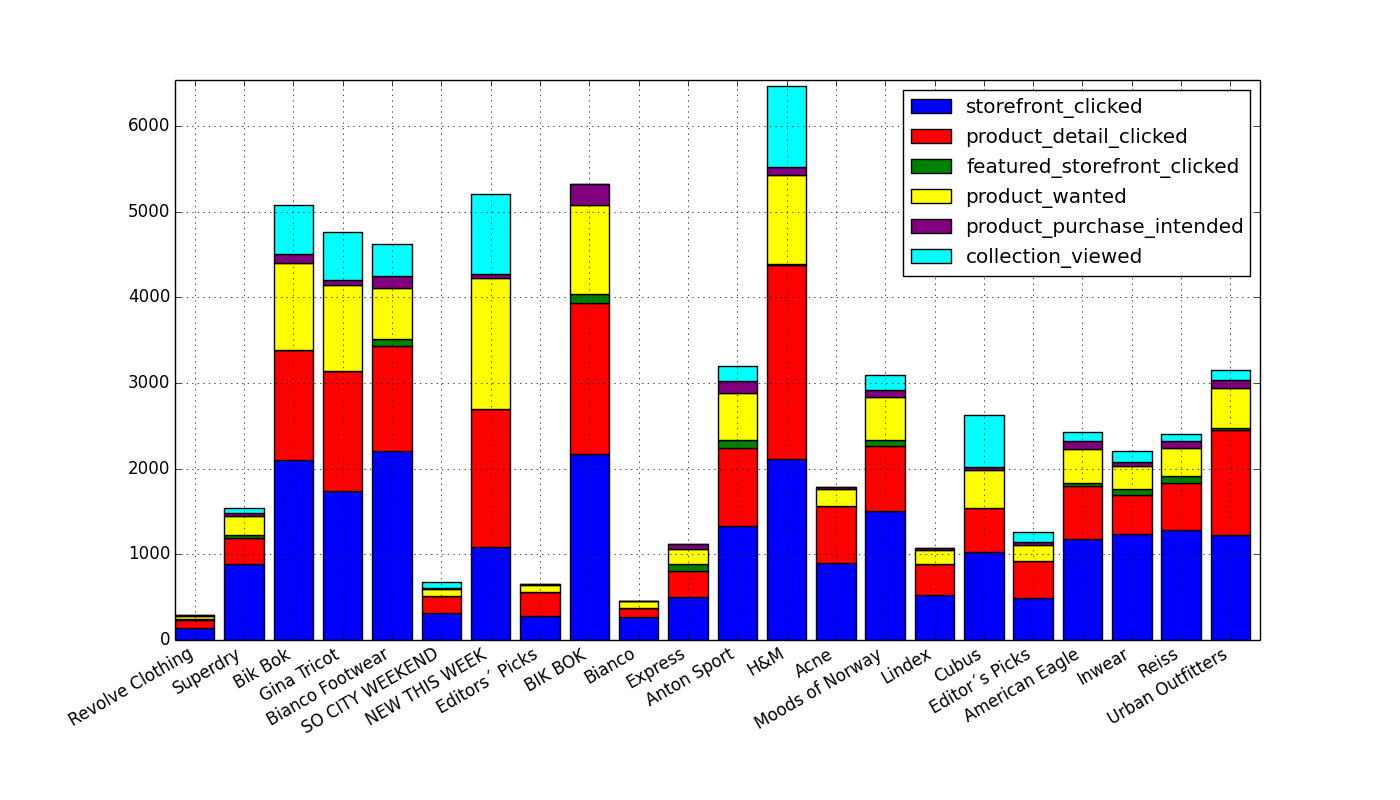
\includegraphics[width=5in]{image/storefront_nameandEventdistribution.png}
  \caption{Distribution of events on storefronts}
  \label{figure:eventOnStoreFrontDist}
\end{figure}

The figure above presents the event distribution on the different storefronts.
The events are segmented to show the different event counts on the different
storefronts, and stacked to show the complete count, to be able to clearly see
how the events are distributed over the different stores.  We can see that
\emph{H\&M} is the most popular store in total, but \emph{BIK BOK} has the most
\emph{product\_purchase\_intended}-events.  One interesting find to take from
this graph is the \emph{storefront\_clicked} to the item interaction related
events (\emph{product\_detail\_clicked}, \emph{product\_wanted} and
\emph{product\_purchase\_intended}) ratio.  For instance \emph{Bik Bok} has a
much higher item interaction count than storefront access count, whereas stores
such as \emph{Reiss} and \emph{Inwear} are mostly accessed and the items not
interacted with.  Different aspects affecting this might be price, style and
item presentation.

\subsection{Time properties}

Not only is it important to look at user and product properties, but as
\textit{time} is an important aspect of fashion we should identify properties
related to this segment in our data as well. We have already looked at the
lifespan of users (Figure~\ref{fig:sessCountDist}), and by applying the same
methodology on products we can see which items that regularily are interacted
with -- and perhaps more interestingly, which items are \textit{forgotten}.

\begin{figure}[H]
  \centering
  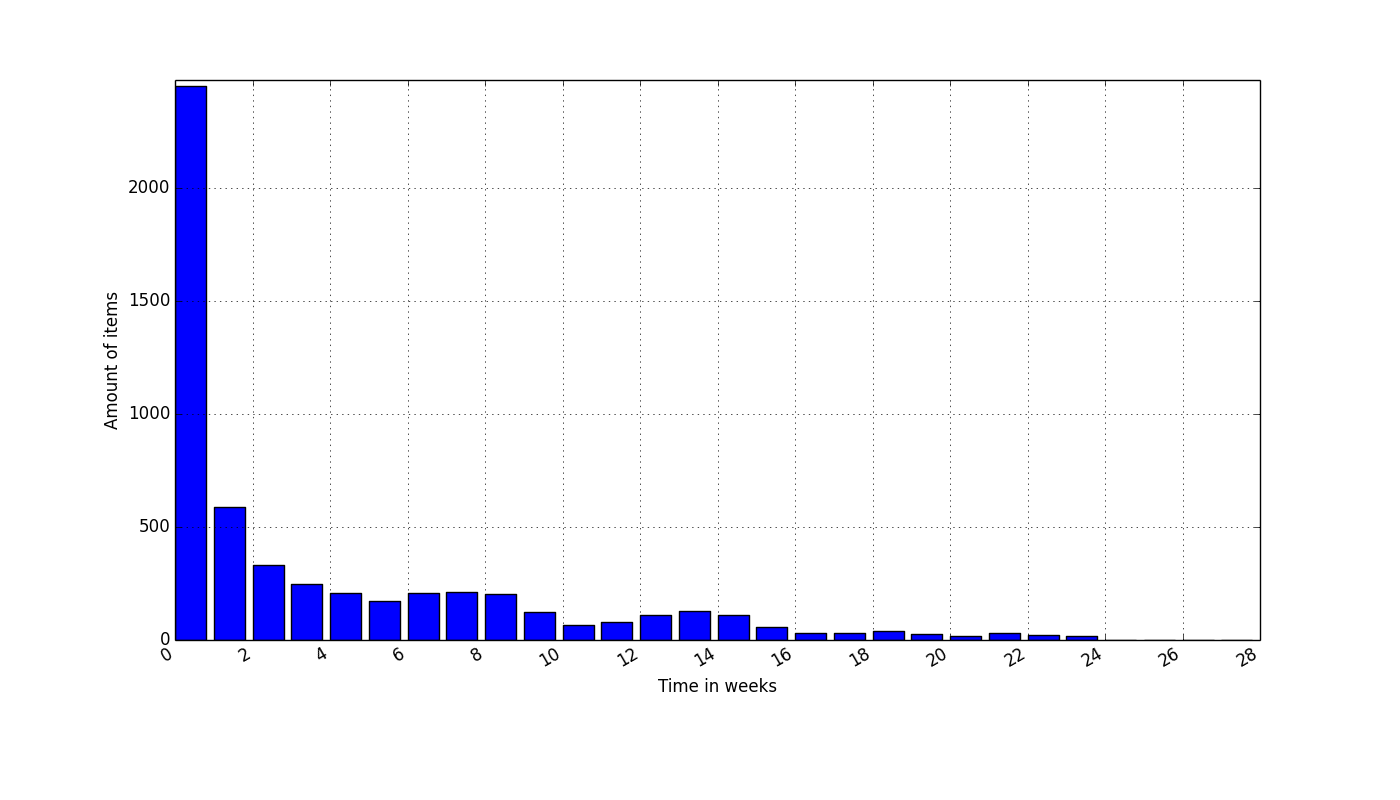
\includegraphics[width=5in]{image/itemTimespansdistribution.png}
  \caption{Count of the different time spans of the items}
  \label{figure:itemLifes}
\end{figure}

We can observe that almost 2 500 products have a life span of less than a week,
which shows how important it is to handle the recentness of products in order
to follow ever-changing trends. In addition, a future recommender system should
strive not only to show the most popular items at moment, but also ensure a
large \textit{coverage} of the product database in its recommendations. This is
an important metric, which we will return to multiple times in this thesis --
since, as we can see the coverage of items in the current state is low.

Increasing the lifespan of an item has positive effects on the popularity of an
item as well, as we see in the figure below, where the lifespan is mapped to
the number of interactions on the item in question.

\begin{figure}[H]
  \centering
  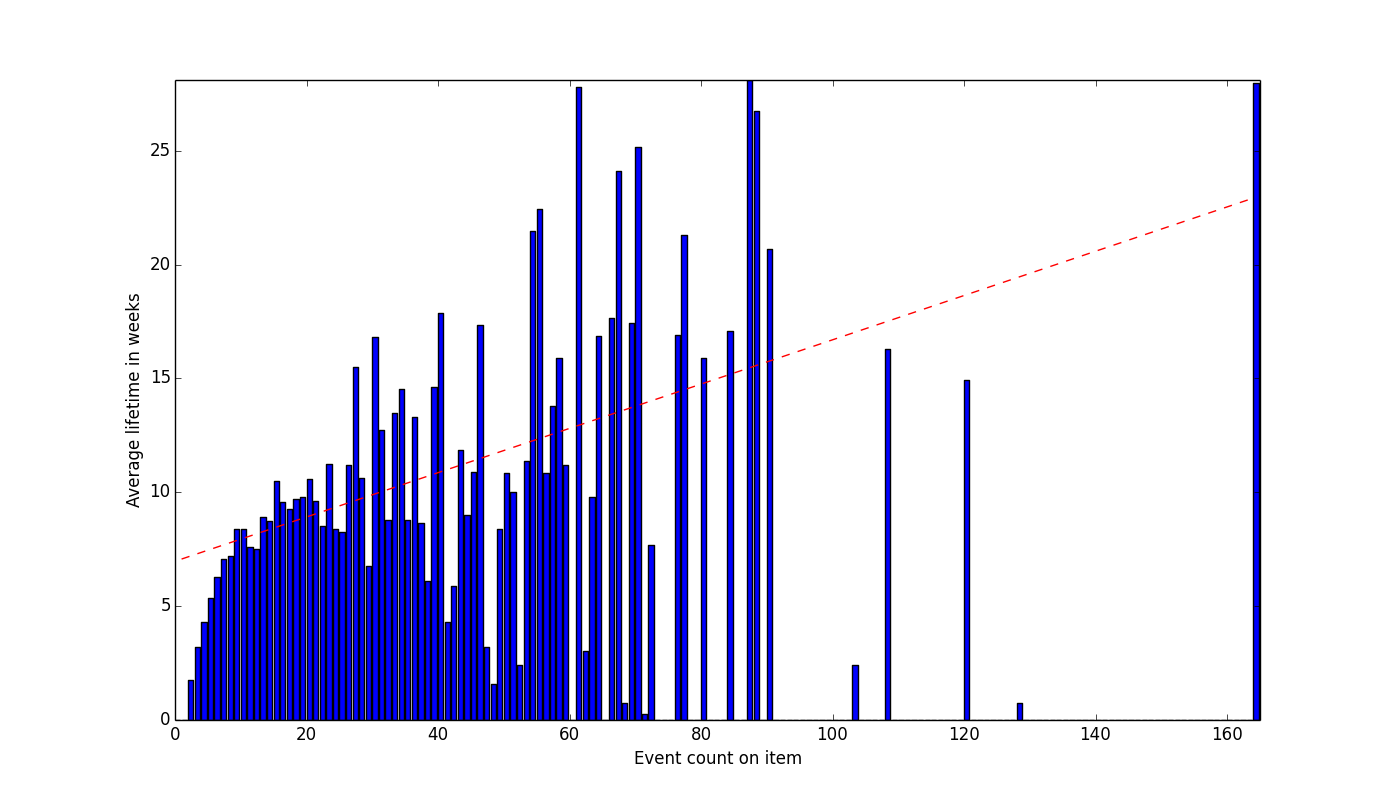
\includegraphics[width=5in]{image/avglifetimeoncount.png}
  \caption{Average life time of products grouped on event count}
  \label{figure:averageLifetimBasedoncount}
\end{figure}

One may see that the tendency line shows a positive growth as the average
number of item interactions increase. Thus, as they are correlated it is both
important to focus on making good recommendations, but also ensure good
coverage. One may also see the sparsity affects this figure, as e.g. no items
have between 116 and 160 interactions registered.

The figure above averaged the lifespan of the items and presented them with
together with their respective count, below we show the same tendency, but keep
the lifespan seperate.

\begin{figure}[H]
  \centering
  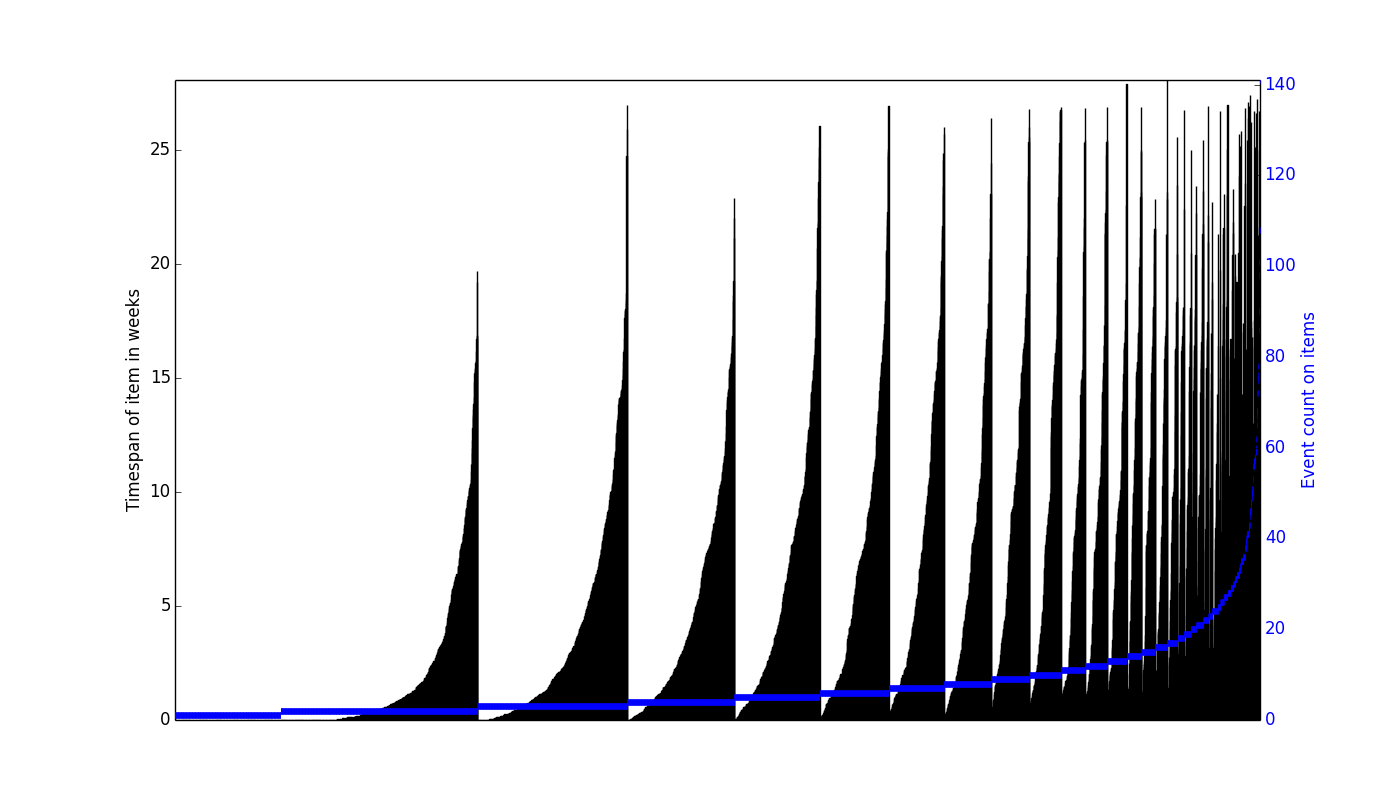
\includegraphics[width=5in]{image/itemTimeSpansortedoneventcount.png}
  \caption{Life time of items mapped with event count}
  \label{figure:itemTimeSpanEventCount}
\end{figure}

Time is shown in weeks, so the longest time span of an item is about 27 weeks,
which is close to the time span of the events gathered from SoBazaar. As can be
seen, even though an item has a long time span, it does not mean that the item
has been of measurable interest to the users in the SoBazaar application. In
addition we see that the more interaction on the item, the longer the average
life time, again proving that the recentness of an item is important.

As described in Section~\ref{sec:preprocessing} when pre-processing the data we
perform a session study, looking at timing related behaviours in order to e.g.
detect the amount of \textit{bouncing}, that is clicking an item and then
without delay return to the original page without \textit{actually} having read
or shown interest to the product.

\begin{figure}[H]
  \centering
  \begin{subfigure}{.5\textwidth}
      \centering
      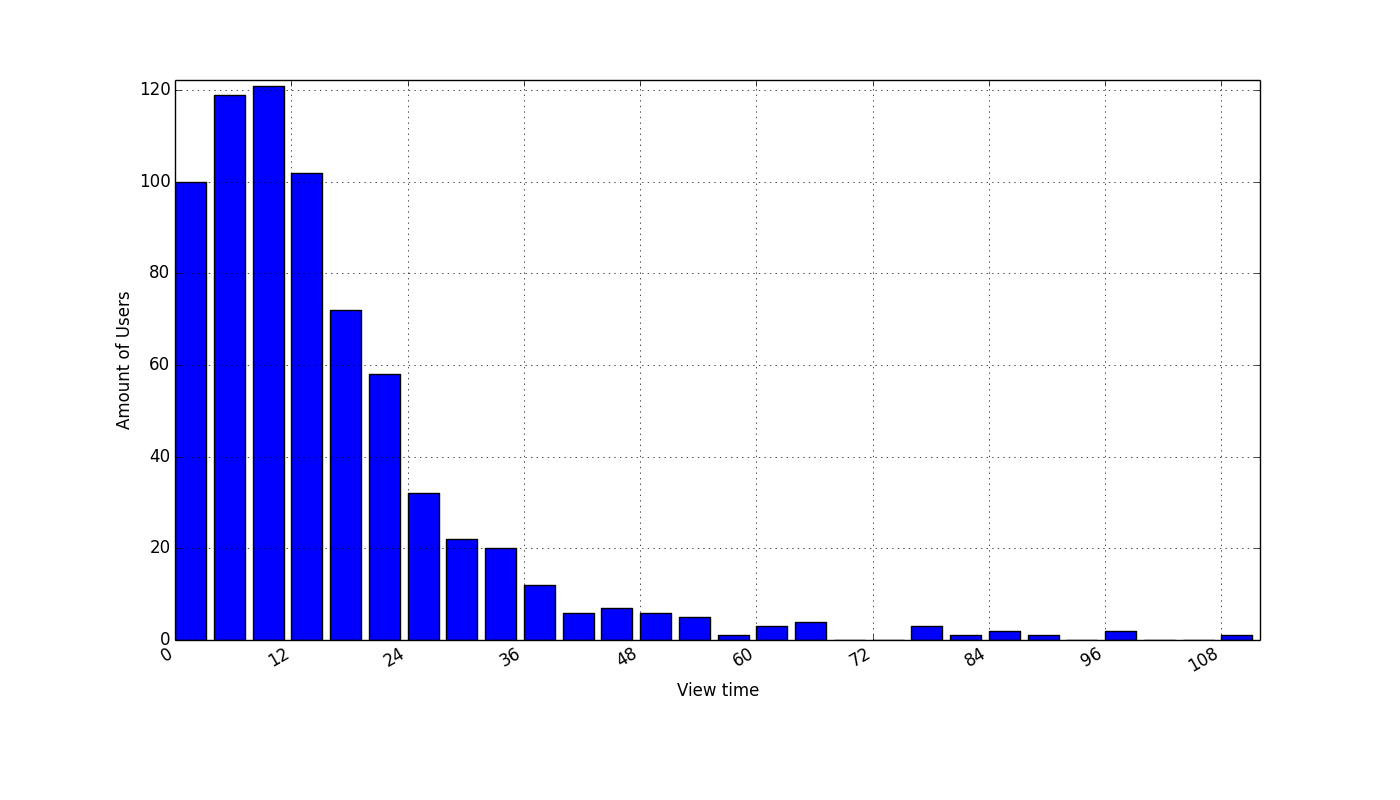
\includegraphics[width=\dualGraphWidth]{image/product_wanteddistribution.png}
      \caption{View times before wanting an item}
      \label{figure:viewWant}
  \end{subfigure}%
  \begin{subfigure}{.5\textwidth}
      \centering
      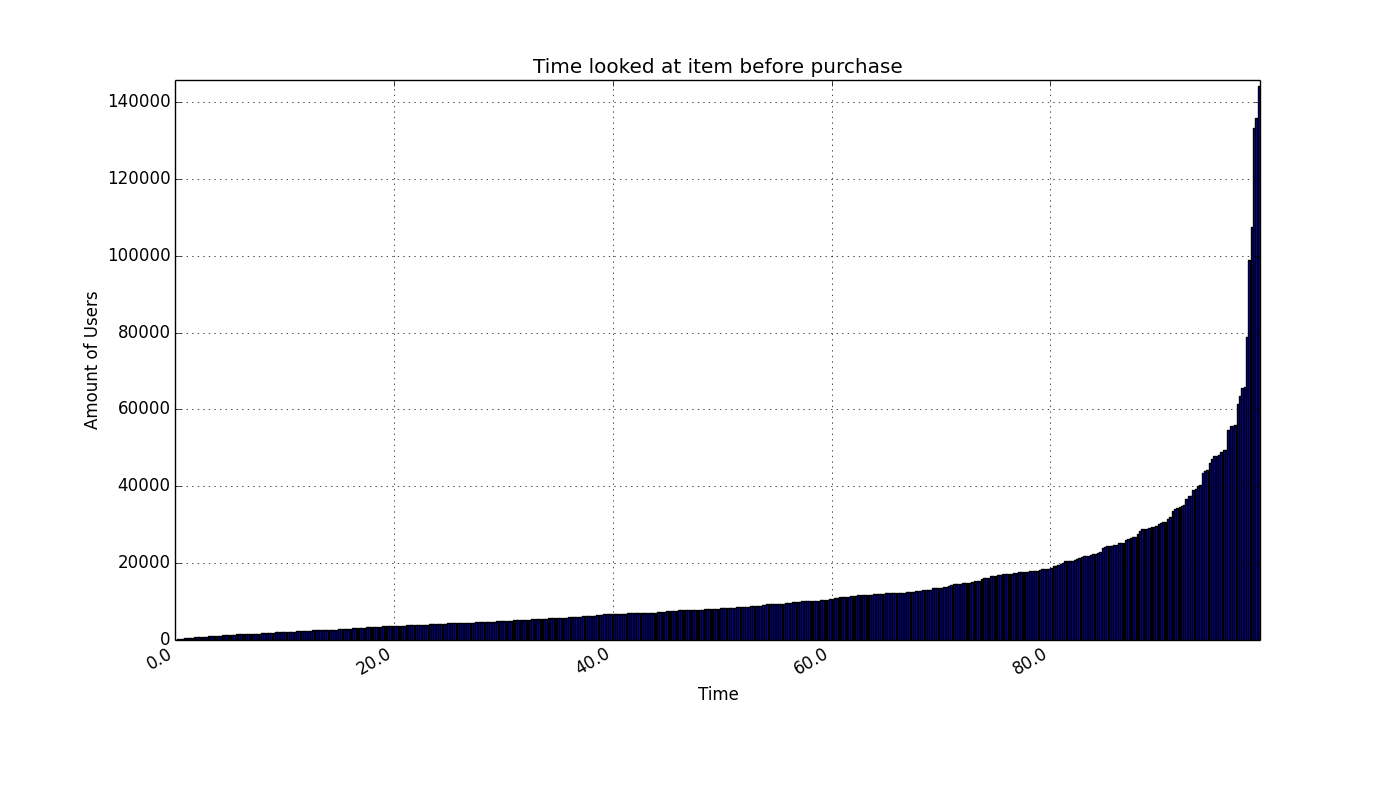
\includegraphics[width=\dualGraphWidth]{image/product_purchase_intendeddistribution.png}
      \caption{View times before purchasing an item}
      \label{figure:viewBuy}
  \end{subfigure}
  \caption{Average view times of products before want or purchase}
  \label{fig:view-times}
\end{figure}

By looking at the average view time before want and purchase above, we conclude
that most users purchases or wants an item by looking at images and perhaps
superficially at the product details. In other words, as we have mentioned
earlier, the most important aspects in terms of retention and conversion are
price, images, status of the item, brand and storefront.

Closely related is the already mentioned \textit{bounce rate}, which is
depicted below.

\begin{figure}[H]
  \centering
  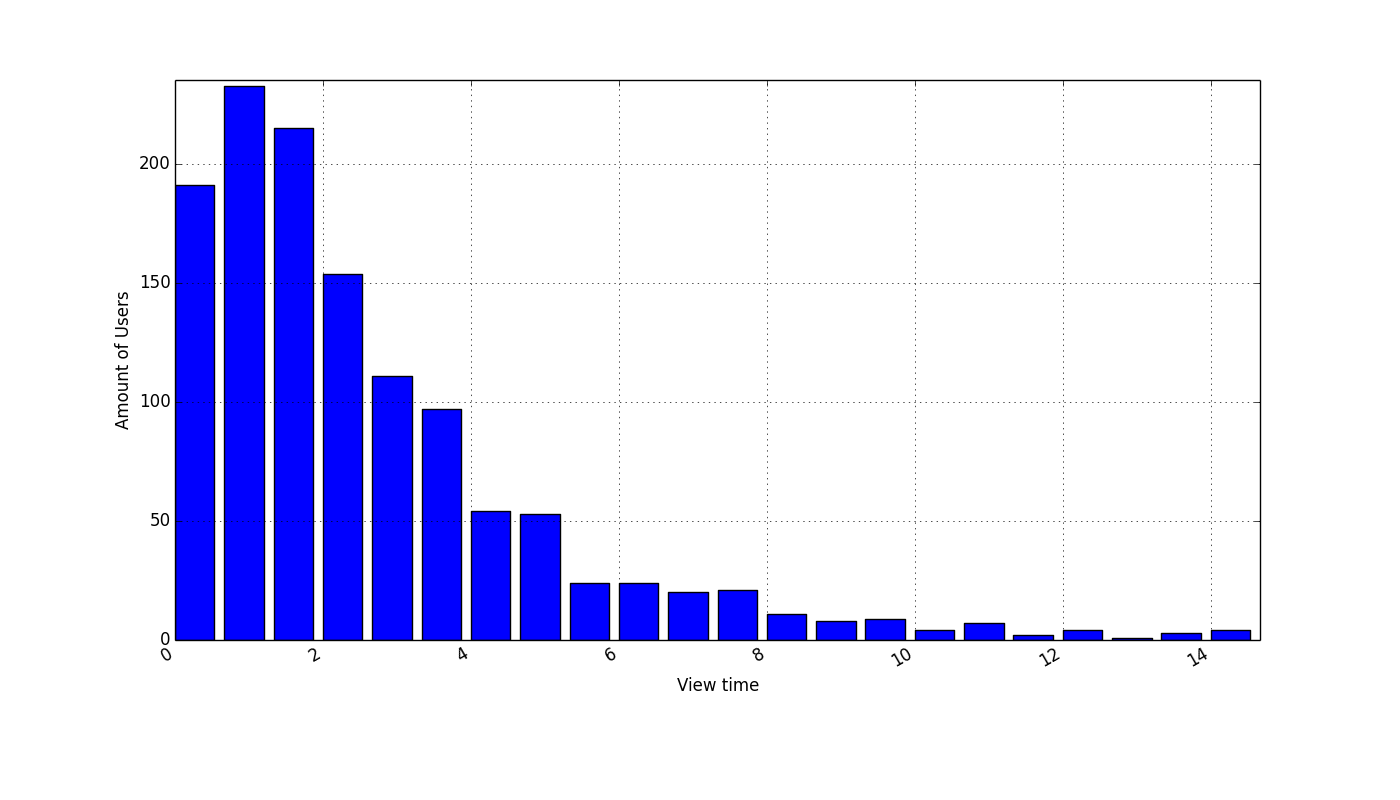
\includegraphics[width=5in]{image/product_detail_clickeddistribution.png}
  \caption{View times before leaving an item (Bounce Rate)}
  \label{figure:bounceRate}
\end{figure}

Comparing the above figure with Figure~\ref{fig:view-times} shows the
difficulty of predicting bounces, as most events are \textit{fast-paced} and
many users both buy and want an item in the same time as other users bounce.
We can however observe that many users leave a product in under 2 seconds, and
this could be used as \textit{negative evidence} in a future recommender --
that is, we should not count it towards understanding the users preferences.

\begin{figure}[H]
  \centering
  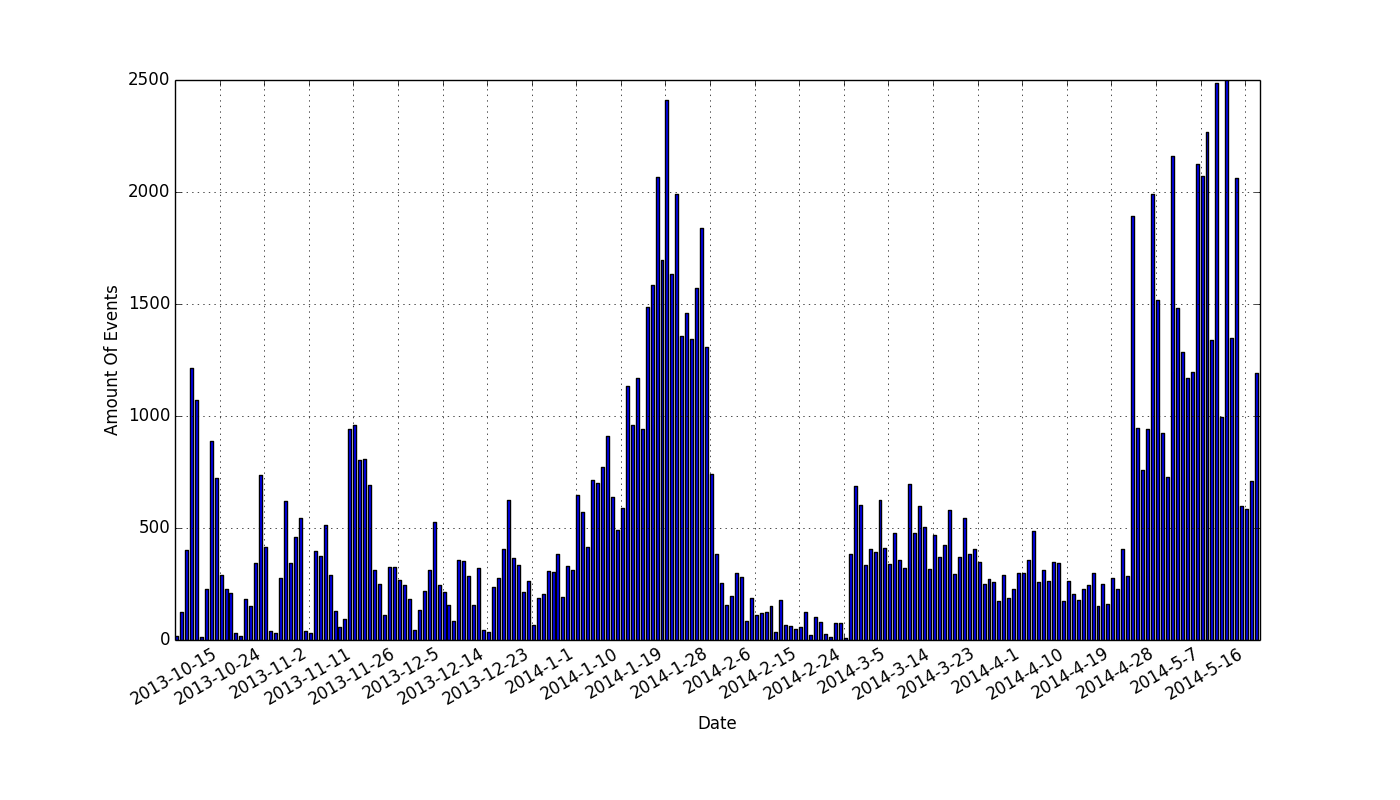
\includegraphics[width=5in]{image/eventsPerDay.png}
  \caption{Distribution of events per day}
  \label{figure:eventOnDaysDist}
\end{figure}

We conclude this section by looking at some key characteristics of the SoBazaar
application in general, namely activity peaks both in terms in the lifespan of
the application and hours of the day. As we can see two activity peaks stand
out, one in mid-January and the second one in May, that is until and including
the last event in the dataset.

However, it is worth mentioning again that the application is not officially
released and thus activity levels are highly sensitive to publicity or other
external factors.

\begin{figure}[H]
  \centering
  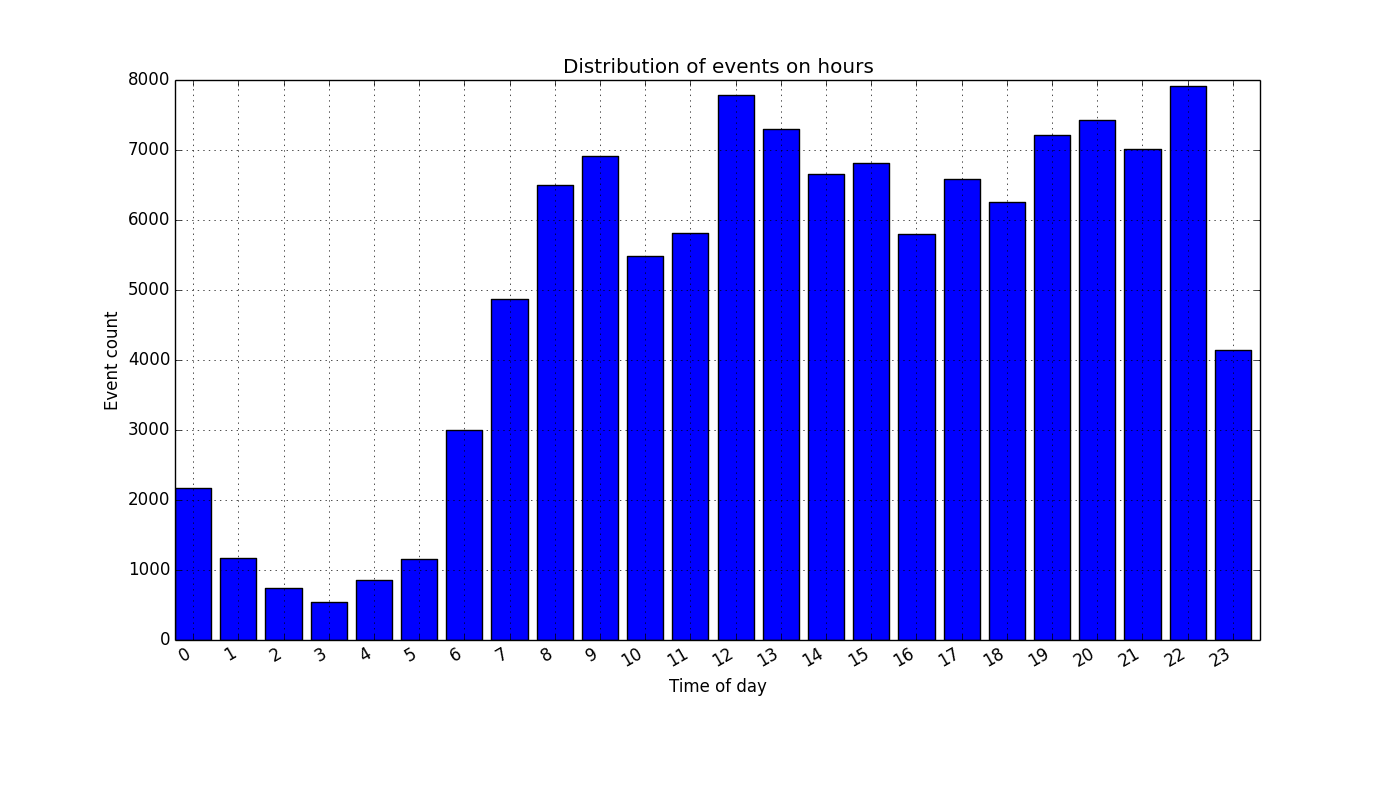
\includegraphics[width=5in]{image/hrdistribution.png}
  \caption{Events at time of day}
  \label{figure:timeOfDayDistr}
\end{figure}

The figure above presents the amount of events during the given hours. One
interesting discovery from this figure is the shape. One might have expected
the application usage to have a sinus wave shape, that is gradually decrease as
we see it does between 15:00 and 16:00. Instead, we see an increase in usage
with a peak around 22:00, which provides strong evidence for SoBazaar primarily
being an entertainment application.

\section{Conversion Rate Properties}
\label{sec:conv-rate}

In many domains the number of activities on an item given a specific user
implies preference. The activity in question may be the number of plays in a
music service~\cite{parra2011walk} or the amount of minutes used watching a
specific TV-show~\cite{Hu2008}. We want to validate this
hypothesis in the SoBazaar data, determining if the \textit{number of clicks}
on an item implies higher preference, that is an higher probability of buying
the item.

If the hypothesis holds true, we can use this fact in order improve
classification of our models in future sections. In addition we can customize
the user interface so that if a user has clicked the item, we should with a
higher frequency show the item to the user -- as he/she is more probable of
buying it once seen in detail.

In order to validate the hypothesis we iterate through all users and look at
their respective events, summarizing the number of times the user has clicked
an item $n$ times and of these how many times the user also bought it. We do
this for all values of $n$, where $n \in [1,6]$ and obtain the following table
of conversion rates and standard errors.

\begin{table}[H]
  \centering
  \begin{tabular}{lllll}
    \toprule
    N & Clicks & Purchases & Rate & Standard Error \\
    \midrule
    1 & 15602 & 1039  & 0.0667 & 0.20\% \\
    2 & 2672  & 323   & 0.1208 & 0.63\% \\
    3 & 433   & 84    & 0.1939 & 1.89\% \\
    4 & 173   & 36    & 0.2081 & 3.10\% \\
    5 & 65    & 19    & 0.2923 & 5.63\% \\
    6 & 54    & 20    & 0.3703 & 6.57\% \\
    \bottomrule
  \end{tabular}
  \caption{Probabilties of purchase, given $N$ visits on item}
  \label{tab:prob-purchase}
\end{table}

The standard error gives a useful indication on how certain we can be that the
results are statistically significant, and is calculated based on the sample
size (number of clicks) and the amount of conversions. Given the rate as $r$
and sample size as $S$ we calculate the standard error $e$ as:

\begin{equation}
  e = \sqrt{\frac{r(1 - r)}{S}}
\end{equation}

Using the standard error we want to perform an hypothesis test determining if
the results are significant within our accepted confidence of 95\%. In other
words we want to be 95\% sure that the patterns found in the data are not just
random. Our two hypothesis which we want to test are thus:

$\mathbf{H_0:}$ The differences in conversion rates between our first
(baseline) and second scenario is random.

$\mathbf{H_1:}$ The difference is significant, such that one scenario have a
higher probability of conversion.

and we want to do multiple tests when $n \in [2,6[$, using $n-1$ as baseline
and $n$ as the second scenario. For each test we calculate the
\textit{P-value}, which is the probability of obtaining a result at least as
extreme as the one that was actually observed. When the P-value becomes less
that our predetermined significance level ($0.05$ when we do a 95\%
significance test) we can reject our null-hypothesis, which is what we want to
do. In order to find this P-value we use the Standard Score, also called the
\textit{Z-score}, which is the number of standard deviations an observation is
above the mean. As we have two samples we can calculate the difference in
conversion rates and use the cumulated standard error in order to find the
Z-score:

\begin{equation}
  \label{eq-z-score}
  Z = \frac{r_b - r_v}{\sqrt{e_{b}^{2} + e_{v}^{2}}}
\end{equation}

where $r_b$ and $r_v$ are the conversion rates for the baseline and second
scenario respecivly. $e_b$ and $e_v$ are equally the standard errors for the
two scenarios. Using standard normal deviate (normallly distributed random
variable with expected value 0 ($s$) and standard deviation 1 ($h$)) we can
find the cumulative probability for validity of the model - the P-value.

We calculate the P-value using $n=1$ as baseline and $n=2$ as our second
scenario. The Z-score is calculated by Equation~\ref{eq-z-score} and we obtain
our result:

\begin{equation}
  Z = \frac{0.0667-0.1208}{\sqrt{0.0020^2 + 0.0063^2}} = \frac{-0.05}{\sqrt{0.4369}} = -8.1848
\end{equation}

This is a very low Z-score, and when we are this many standard deviations away
from the mean in a standard normal deviate the P-value or area under the curve
is approximated to 0. This is a value lower than our predetermined significance
level ($0.05$) and thus we can reject the null-hypothesis and state with
statistical accuracy and correctness that there is a higher probability of
buying the item given that the user has clicked on the item twice, rather than
having clicked on the item only once. In our first scenarios we have sufficient
data to come to this conclusion, however, when comparing later scenarios we see
that our numbers stop being significant as a result of the dataset being too
small.

\begin{table}[H]
  \centering
  \begin{tabular}{lllll}
  \toprule
  Baseline & Alternative & Z-score & P-value & Significant \\
  \midrule
  1 & 2 & -8.1848 & 0.0000 & \cmark \\
  2 & 3 & -3.6516 & 0.0001 & \cmark \\
  3 & 4 & -0.3889 & 0.3487 & \xmark \\
  4 & 5 & -1.3096 & 0.0952 & \xmark \\
  5 & 6 & -0.9013 & 0.1837 & \xmark \\
  \bottomrule
  \end{tabular}
\end{table}

Our conclusion is then that when a user has clicked on an item two times there
is a higher probability of buying it compared to when the user has only
clicked it once. This is also true when the user has clicked an item three
times, but we can not defend it statistically for any higher value of clicks.

\section{Session Patterns}
\label{sec:sessionPatterns}

Since the SoBazaar data is based on the events of the application user, sessions can be constructed from the data.
Sessions are the set of events triggered during one separate user usage of the application.
For instance:

\begin{enumerate}
  \item User logs into the application
  \item User enters a storefront
  \item User clicks an item
  \item User clicks \emph{want} on an item
\end{enumerate}

As seen from the example above, first the user logs inn, which is the trigger flag to indicate a sessions is started. Then user does a set of actions in the application.
These events put together forms the a session of a user and is used in the figure below to better understand the global user patterns.

\begin{figure}[H]
  \centering
  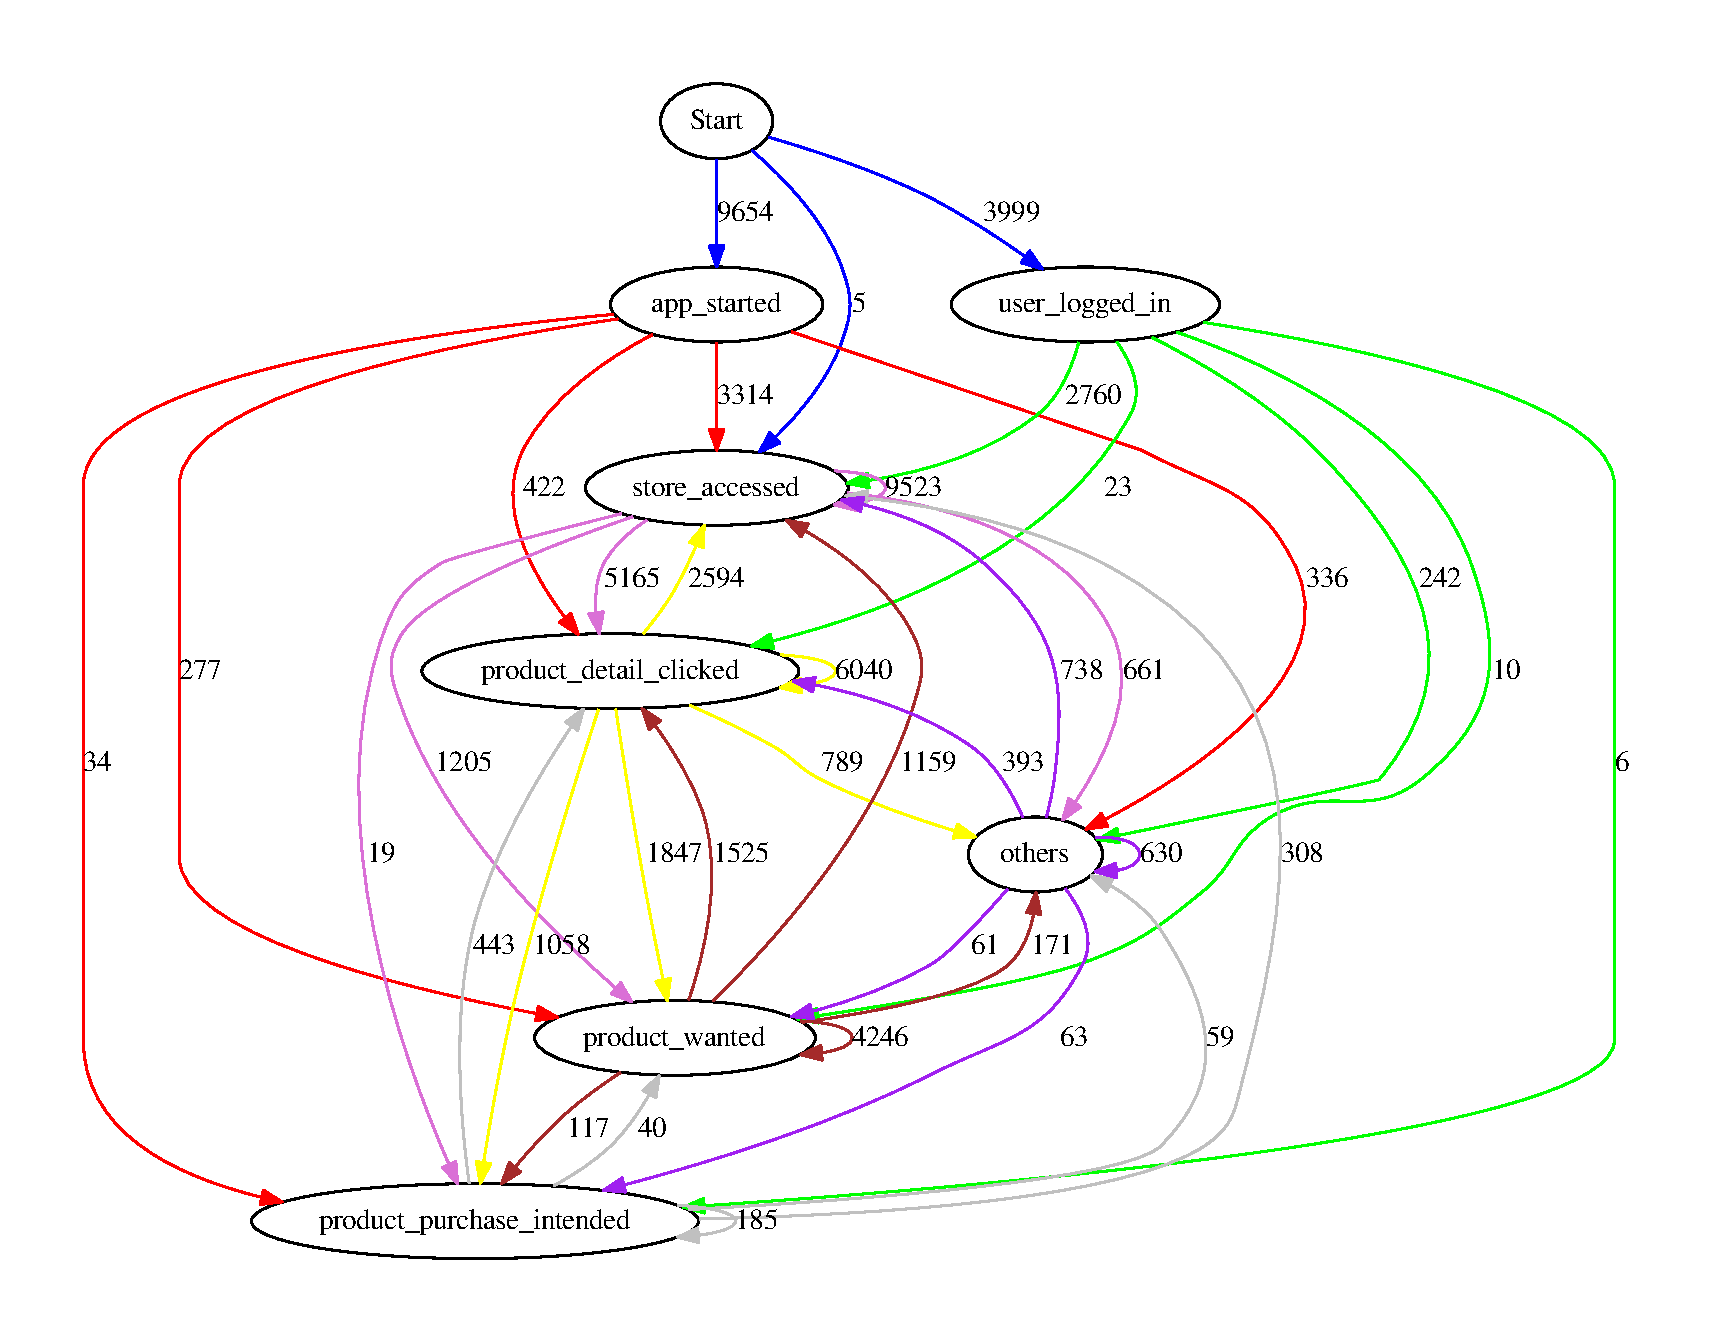
\includegraphics[width=5in]{image/statesInteractionTrue-gvfile.pdf}
  \caption{A minimized view of the different states of the system and how they interact with each other.}
  \label{figure:minStatesInteractions}
\end{figure}

The figure above presents the events as states and shows the interactions
between them.  The weights on the edges between the states are the count of
state changes from the sending state to the receiving state.  As we can see
from the figure, states can access themselves.  This figure is a minimized view
to better present the state interactions regarding products, where states such
as \emph{activity\_clicked}, \emph{around\_me\_clicked} and
\emph{stores\_map\_clicked}, have been left out to give focus to item
interaction related states.

For a more complete view without reduced states see~\ref{figure:statesInteractions}.

The \emph{Init}-state is the initialization of the application, which leads to
the \emph{Start}-state, which is a reduction of the variations of events which
indicates that a session is started, such as \emph{user\_logged\_in},
\emph{app\_started} and \emph{app\_first\_started}.  From this most of the
users enter the \emph{store\_accessed}-state, which is the shared state of all
the store related states.

As we can see from the figure, in 9 470 cases the users enters a store after
already having entered a store, which means that the user did not access any of
the items in the first entered store, and we see that this is a common way of
browsing the products in the application. Since this leaves little indication
about the user preferences, other ways of gathering this must be utilized.
While this thesis was being written additional events was added, one of these
was \emph{content:interact:item\_scroll}, which has proven to be of good help
to derive user preferences~\cite{Claypool01inferringuser}.

If we focus on the states \emph{product\_wanted} and
\emph{product\_purchase\_intended}, we see that 144 occurrences of being in the
\emph{product\_wanted}-state progressed into the
\emph{product\_purchase\_intended}-state.

Based on the information above we better see that storefront related events and browsing them are a quite normal behavior, as expected after we saw Figure~\ref{figure:eventIDDistribution}, but we also see that the most often occurring next state after doing a \emph{product\_detail\_clicked} is another \emph{product\_detail\_clicked}, which indicates a sense of store belonging from the user.
This can also be seen by the fact that there are 5 755 entries into \emph{product\_detail\_clicked} from a store access, but only 3 134 out. And this is true even though there are 1 596 store accesses after a \emph{product\_wanted} event since there are so many \emph{product\_wanted} events after store accesses.

One interesting find is that the most occurring way of accessing a \emph{product\_detail\_clicked} state, is by just having been in a \emph{product\_detail\_clicked} state, which strengthens the hypothesis that users are brand aware.
